%% abtex2-modelo-trabalho-academico.tex, v-1.9.3 laurocesar
%% Copyright 2012-2015 by abnTeX2 group at http://abntex2.googlecode.com/ 
%% This work may be distributed and/or modified under the
%% conditions of the LaTeX Project Public License, either version 1.3
%% of this license or (at your option) any later version.
%% The latest version of this license is in
%%   http://www.latex-project.org/lppl.txt
%% and version 1.3 or later is part of all distributions of LaTeX
%% version 2005/12/01 or later.
%%
%% This work has the LPPL maintenance status `maintained'.
%% 
%% The Current Maintainer of this work is the abnTeX2 team, led
%% by Lauro César Araujo. Further information are available on 
%% http://abntex2.googlecode.com/
%%
%% This work consists of the files abntex2-modelo-trabalho-academico.tex,
%% abntex2-modelo-include-comandos and abntex2-modelo-references.bib
%%

% ------------------------------------------------------------------------
% ------------------------------------------------------------------------
% abnTeX2: Modelo de Trabalho Academico (tese de doutorado, dissertacao de
% mestrado e trabalhos monograficos em geral) em conformidade com 
% ABNT NBR 14724:2011: Informacao e documentacao - Trabalhos academicos -
% Apresentacao
% ------------------------------------------------------------------------
% ------------------------------------------------------------------------

\documentclass[
	% -- opções da classe memoir --
	12pt,				% tamanho da fonte
	openright,			% capítulos começam em pág ímpar (insere página vazia caso preciso)
	twoside,			% para impressão em verso e anverso. Oposto a oneside
	a4paper,			% tamanho do papel. 
	% -- opções da classe abntex2 --
	chapter=TITLE,		% títulos de capítulos convertidos em letras maiúsculas
	%section=TITLE,		% títulos de seções convertidos em letras maiúsculas
	%subsection=TITLE,	% títulos de subseções convertidos em letras maiúsculas
	%subsubsection=TITLE,% títulos de subsubseções convertidos em letras maiúsculas
	% -- opções do pacote babel --
	english,			% idioma adicional para hifenização
	brazil				% o último idioma é o principal do documento
	]{abntex2}

% ---
% Pacotes básicos 
% ---
% \usepackage{uarial}				% Usa a fonte Latin Modern			lmodern
\usepackage[T1]{fontenc}		% Selecao de codigos de fonte.
\usepackage[utf8]{inputenc}		% Codificacao do documento (conversão automática dos acentos)
\usepackage{lastpage}			% Usado pela Ficha catalográfica
\usepackage{indentfirst}		% Indenta o primeiro parágrafo de cada seção.
\usepackage{color}				% Controle das cores
\usepackage{graphicx}			% Inclusão de gráficos
\usepackage{microtype} 			% para melhorias de justificação
\usepackage{longtable}
\usepackage{multirow}
% pacotes adicionados
\usepackage{amsmath}
\usepackage{amssymb,amsfonts,amsthm}
\usepackage{setspace}
%\usepackage{geometry}

% --- pacote para inserir documentos PDF
\documentclass[a4paper]{article}
\usepackage[utf8]{inputenc}
\usepackage[T1]{fontenc}
\usepackage[brazil]{babel}
\usepackage{pdfpages}
		
% ---
% Pacotes adicionais, usados apenas no âmbito do Modelo Canônico do abnteX2
% ---
\usepackage{lipsum}				% para geração de dummy text
% ---
\usepackage{todonotes}
% ---
% Pacotes de citações
% ---
\usepackage[brazilian,hyperpageref]{backref}	 % Paginas com as citações na bibl
\usepackage[alf]{abntex2cite}	% Citações padrão ABNT


\renewcommand{\bf}[1]{\mathbf{#1}}
\renewcommand{\rm}[1]{\mathrm{#1}}

\usepackage{graphicx}
\usepackage{subfig}

\usepackage{cite}
\renewcommand\citeleft{}
\renewcommand\citeright{}

% --- 
% CONFIGURAÇÕES DE PACOTES
% --- 
\renewcommand{\imprimircapa}{
\thispagestyle{empty}

\vfill
 \begin{center}

    \begin{figure}
	   \centering
	   		
\includegraphics[scale=0.35]{figs/brasao_uesc.png}
    \end{figure}

    {\large\bfseries UNIVERSIDADE ESTADUAL DE SANTA CRUZ - UESC} \\


    {\large\bfseries DEPARTAMENTO DE CIÊNCIAS EXATAS E TECNOLÓGICAS}  \\

    \vspace*{1in}
    \begin{large} \bfseries Alexandre Pedrecal Campos \end{large}\\[0.4in]

    \vspace*{4cm}
    \noindent \\

    \large\bfseries{\begin{large}DESENVOLVIMENTO DE API PARA EXTRAÇÃO DE INFORMAÇÃO TEXTUAL DE ARQUIVOS PDF PADRONIZADOS\end{large}} \\
    % \large\bfseries{\begin{large}DESENVOLVIMENTO DE API PARA EXTRAÇÃO AUTOMÁTICA DE INFORMAÇÕES DE ARQUIVOS PDF APLICADA A TRABALHOS DE CONCLUSÃO DE CURSO\end{large}} \\
    \vfill
    \large\bfseries{ ILHÉUS - BAHIA \\ 2020}
\end{center}

\normalsize


}

\usepackage{multirow}

\renewcommand{\imprimirfolhaderosto}{

\begin{center}

    {\large \begin{large} \bfseries ALEXANDRE PEDRECAL CAMPOS \end{large}\\}
    \vspace{8cm}
    {\large\bfseries{\begin{large}DESENVOLVIMENTO DE API PARA EXTRAÇÃO DE INFORMAÇÃO TEXTUAL DE ARQUIVOS PDF PADRONIZADOS\end{large}}\\}
    % {\large\bfseries{\begin{large}DESENVOLVIMENTO DE API PARA EXTRAÇÃO AUTOMÁTICA DE INFORMAÇÕES DE ARQUIVOS PDF APLICADA A TRABALHOS DE CONCLUSÃO DE CURSO\end{large}}\\}
    \vspace{1cm}
    \hspace{.45\linewidth}
    \begin{minipage}{.50\linewidth}
            Trabalho de Conclusão de Curso apresentado à Universidade Estadual de Santa Cruz - UESC, como parte das exigências para obtenção do título de Bacharel em Ciência da Computação.
            \\ Orientador: Prof. Mestre Hélder Conceição Almeida


    \end{minipage}

    \vspace{2cm}
    \vfill
    {\large\bfseries{ ILHÉUS - BAHIA \\ 2020}}
\end{center}

}


% ---
% Configurações do pacote backref
% Usado sem a opção hyperpageref de backref
\renewcommand{\backrefpagesname}{Citado na(s) página(s):~}
% Texto padrão antes do número das páginas
\renewcommand{\backref}{}
% Define os textos da citação
\renewcommand*{\backrefalt}[4]{
	\ifcase #1 %
		Nenhuma citação no texto.%
	\or
		Citado na página #2.%
	\else
		Citado #1 vezes nas páginas #2.%
	\fi}%
% ---
% ---
% Informações de dados para CAPA e FOLHA DE ROSTO
% ---

\titulo{}
\autor{}
\local{Brasil}
\data{2018, v-1.9.3}
\orientador{}
%\coorientador{coorientador}
\instituicao{%
  Universidade Estadual de Santa Cruz UESC
  \par
  Departamento de Ciências Exatas e Tecnológicas
  }
\tipotrabalho{Projeto de Fim de Curso}
% O preambulo deve conter o tipo do trabalho, o objetivo, 
% o nome da instituição e a área de concentração 
\preambulo{O preambulo deve conter o tipo do trabalho, o objetivo, o nome da instituição e a área de concentração }
% ---






% ---
% Configurações de aparência do PDF final

% alterando o aspecto da cor azul
\definecolor{blue}{RGB}{41,5,195}

% informações do PDF
\makeatletter
\hypersetup{
     	%pagebackref=true,
		colorlinks=false,       		% false: boxed links; true: colored links
    	linkcolor=blue,          	% color of internal links
    	citecolor=black,        		% color of links to bibliography
    	filecolor=magenta,      		% color of file links
		urlcolor=blue,
		bookmarksdepth=4
}



\makeatother
% ---




% --- 
% Espaçamentos entre linhas e parágrafos 
% --- 



% O tamanho do parágrafo é dado por:
\setlength{\parindent}{1.3cm}

% Controle do espaçamento entre um parágrafo e outro:
\setlength{\parskip}{0.2cm}  % tente também \onelineskip

% ---
% compila o indice
% ---
\makeindex
% ---

% ----
% Início do documento
% ----
\usepackage{float}
\usepackage{svg}

\begin{document}

% Seleciona o idioma do documento (conforme pacotes do babel)
%\selectlanguage{english}
\selectlanguage{brazil}

% Retira espaço extra obsoleto entre as frases.
\frenchspacing 

% ----------------------------------------------------------
% ELEMENTOS PRÉ-TEXTUAIS
% ----------------------------------------------------------
\pretextual

% ---
% Capa
% ---
\imprimircapa
% ---

% ---
% Folha de rosto
% (o * indica que haverá a ficha bibliográfica)
% ---
\imprimirfolhaderosto

% ---
% Inserir a ficha bibliografica
% ---

% Isto é um exemplo de Ficha Catalográfica, ou ``Dados internacionais de
% catalogação-na-publicação''. Você pode utilizar este modelo como referência. 
% Porém, provavelmente a biblioteca da sua universidade lhe fornecerá um PDF
% com a ficha catalográfica definitiva após a defesa do trabalho. Quando estiver
% com o documento, salve-o como PDF no diretório do seu projeto e substitua todo
% o conteúdo de implementação deste arquivo pelo comando abaixo:
%
% \begin{fichacatalografica}
%     \includepdf{fig_ficha_catalografica.pdf}
% \end{fichacatalografica}

\begin{fichacatalografica}
%	\sffamily
%	\vspace*{\fill}					% Posição vertical
%	\begin{center}					% Minipage Centralizado
%	\fbox{\begin{minipage}[c][8cm]{13.5cm}		% Largura
%	\small
%	\imprimirautor
%	%Sobrenome, Nome do autor
%	
%	\hspace{0.5cm} \imprimirtitulo  / \imprimirautor. --
%	\imprimirlocal, \imprimirdata-
%	
%	\hspace{0.5cm} \pageref{LastPage} p. : il. (algumas color.) ; 30 cm.\\
%	
%	\hspace{0.5cm} \imprimirorientadorRotulo~\imprimirorientador\\
%	
%	\hspace{0.5cm}
%	\parbox[t]{\textwidth}{\imprimirtipotrabalho~--~\imprimirinstituicao,
%	\imprimirdata.}\\
%	
%	\hspace{0.5cm}
%		1. Palavra-chave1.
%		2. Palavra-chave2.
%		2. Palavra-chave3.
%		I. Orientador.
%		II. Universidade xxx.
%		III. Faculdade de xxx.
%		IV. Título 			
%	\end{minipage}}
%	\end{center}
\end{fichacatalografica}
%% ---
% Inserir errata
% ---
\begin{errata}
Elemento opcional da \citeonline[4.2.1.2]{NBR14724:2011}. Exemplo:

\vspace{\onelineskip}

FERRIGNO, C. R. A. \textbf{Tratamento de neoplasias ósseas apendiculares com
reimplantação de enxerto ósseo autólogo autoclavado associado ao plasma
rico em plaquetas}: estudo crítico na cirurgia de preservação de membro em
cães. 2011. 128 f. Tese (Livre-Docência) - Faculdade de Medicina Veterinária e
Zootecnia, Universidade de São Paulo, São Paulo, 2011.

\begin{table}[htb]
\center
\footnotesize
\begin{tabular}{|p{1.4cm}|p{1cm}|p{3cm}|p{3cm}|}
  \hline
   \textbf{Folha} & \textbf{Linha}  & \textbf{Onde se lê}  & \textbf{Leia-se}  \\
    \hline
    1 & 10 & auto-conclavo & autoconclavo\\
   \hline
\end{tabular}
\end{table}

\end{errata}
% ---

% ---
% Inserir folha de aprovação
% ---

% Isto é um exemplo de Folha de aprovação, elemento obrigatório da NBR
% 14724/2011 (seção 4.2.1.3). Você pode utilizar este modelo até a aprovação
% do trabalho. Após isso, substitua todo o conteúdo deste arquivo por uma
% imagem da página assinada pela banca com o comando abaixo:
%
% \includepdf{folhadeaprovacao_final.pdf}
%
\begin{folhadeaprovacao}


\begin{center}
    % Novo

    {\large \begin{large} \bfseries ALEXANDRE PEDRECAL CAMPOS \end{large}\\}
    \vspace{4cm}
    {\large\bfseries{\begin{large} Trabalho de Conclusão de Curso apresentado à Universidade Estadual de Santa Cruz - UESC, como parte das exigências para obtenção do título de Bacharel em Ciência da Computação. \end{large}}\\}
    \vspace{1cm}
    \hspace{.45\linewidth}
    \begin{minipage}{.50\linewidth}

            Trabalho de Conclusão de Curso apresentado à Universidade Estadual de Santa Cruz - UESC, como parte das exigências para obtenção do título de Bacharel em Ciência da Computação.
    \end{minipage}
    \\
\end{center}
    \textbf{Ilhéus, 26 de Agosto de 2019}
\begin{center}
            % {UNIVERSIDADE ESTADUAL DE SANTA CRUZ} \\


    % \vspace{1.5cm}
    %                                 {\begin{large} \bfseries \end{large}}\\
    \bfseries{}
\end{center}

    \vspace{2.5cm}
    \assinatura{Prof. Mestre Hélder Conceição Almeida \\ UESC/DCET \\ (Orientador)}
    \assinatura{Prof. Doutor Marcelo Ossamu Honda \\ UESC/DCET }
    % \assinatura{Prof. Doutor Marcílio Ferreira Marques Filho \\ UESC/DCS }
    \vspace{3 cm}%\vfill

    % \begin{center}
    %     Ilhéus, 06 de julho de 2018
    % \end{center}

\end{folhadeaprovacao}

% ---
% Dedicatória
% ---
\begin{dedicatoria}
   \vspace*{\fill}
   \centering
   \noindent
   \textit{Dedico esse trabalho aos meus pais Edvaldo e Eudalia pelo apoio e incentivo concedidos todos estes anos, ao meu irmão Otávio e a toda minha família e amigos que contribuíram nessa jornada.} \vspace*{\fill}
\end{dedicatoria}
% ---

% ---
% Agradecimentos
% ---
\begin{agradecimentos}
Agradeço primeiramente a Deus, por ter-me concedido saúde e sabedoria, permitindo assim a realização das atividades durante minha graduação.

Agradeço a todos os meus familiares que me apoiaram e me ajudaram no momentos difíceis. Em especial a minha prima Erika e seu Esposo Raul, por ter me acolhido na sua residência todos esses anos. E por todo o carinho e cuidado que tiveram comigo.  

À Universidade Estadual de Santa Cruz (UESC) pela infraestrutura e bolsas de Iniciação Científica concedidas.

À todos os professores que participaram da minha graduação. Ao Professor Esbel Tomás, pela orientação e suporte dados na elaboração desse trabalho. Pelo projeto de iniciação cientifica a mim confiado. Por todas as experiências, conhecimentos e concelhos concedidos. Ao Professor Jauberth Abijaude, com quem tive o privilégio de trabalhar. E ao Professor Marcelo Ossamu Honda, por todas as instruções e cobranças para as etapas de construção do TCC.

À todos envolvidos no desenvolvimento do ETHEL, principalmente ao meu amigo e colega de iniciação científica Raí Bizerra que teve participação direta no desenvolvimento desse trabalho.

Aos pesquisadores Sabrina Martins e Marcílio Ferreira que cederam dados essenciais para elaboração desse trabalho.

Ao Núcleo de Biologia Computacional e Gestão de Informações Biotecnológicas (NBCGIB) pela infraestrutura disponibilizada para o desenvolvimento de projetos durante minha graduação.

Os meus amigos Gabriel Figueiredo, Levy Marlon, Adson Cardoso, Aurélio Chaussê, Gabriel Rodrigues, Matheus Almeida, Alexandre Pedrecal, Alberto Segundo e Daniel Penedo que foram verdeiros irmãos durante essa jornada.







\end{agradecimentos}
% ---
%% ---
% Epígrafe
% ---
\begin{epigrafe}
    \vspace*{\fill}
	\begin{flushright}
\textit{}
	\end{flushright}
\end{epigrafe}
% ---

% ---
% RESUMOS
% ---

% resumo em português
\setlength{\absparsep}{18pt} % ajusta o espaçamento dos parágrafos do resumo
\begin{resumo}
Para permitir a aplicação de protocolos de posturografia utilizando a \textit{Wii Balance Board} (WBB; Nintendo, Kyoto, Japão), um grupo de pesquisadores da Universidade Estadual de Santa Cruz (UESC) são responsáveis pela produção do sistema ETHEL, que já conta com um protótipo em estagio avançado de desenvolvimento. Antes de passar para a etapa de testes clínicos com pacientes é necessário à validação dos resultados obtidos com o ETHEL. Sendo assim, o presente trabalho propõe %fazer um estudo 
uma metodologia para fazer um estudo comparativo dos softwares ETHEL e \textit{Posturography Test}, desenvolvido pelo grupo \textit{Neurorehabilitation \& Brain Research Group},  que já foi testado e validado como ferramenta para realização de testes de avaliação clínica para controle de postura e de equilíbrio, utilizando a WBB. %O estudo tem como objetivo validar os resultados obtidos com o ETHEL. 
Para realização do estudo comparativo foram aprimorados e desenvolvidos protocolos no ETHEL, com intuito de reproduzir as métricas utilizadas pelo \textit{Posturography Test}. Como resultado temos uma técnica que deve permitir corroborar a metodologia de calibração e obtenção dos dados no o ETHEL, assim como otimizar os protocolos de medição. Desta forma disponibilizamos um protótipo que pode ser utilizado para um estudo comparativo dos softwares ETHEL e \textit{Posturography Test}.
\vspace{\onelineskip}
 
\noindent 
Palavras-chave:  \textit{Wii Balance Board}, Posturografia, \textit{Posturography Test}, ETHEL.
\end{resumo}

% resumo em inglês
%\begin{resumo}[Abstract]
% \begin{otherlanguage*}{english}
 % Realizar a verificação ortográfica, sintaxe e semântica.

 %  \vspace{\onelineskip}
 
  % \noindent 
  % \textbf{Keywords}: 
 %\end{otherlanguage*}
%\end{resumo}

%% resumo em francês 
%\begin{resumo}[Résumé]
% \begin{otherlanguage*}{french}
%    Il s'agit d'un résumé en français.
% 
%   \textbf{Mots-clés}: latex. abntex. publication de textes.
% \end{otherlanguage*}
%\end{resumo}
%
%% resumo em espanhol
%\begin{resumo}[Resumen]
% \begin{otherlanguage*}{spanish}
%   Este es el resumen en español.
%  
%   \textbf{Palabras clave}: latex. abntex. publicación de textos.
% \end{otherlanguage*}
%\end{resumo}
% ---

% ---
% inserir lista de ilustrações
% ---
\pdfbookmark[0]{\listfigurename}{lof}
\listoffigures*
\cleardoublepage
%% ---

% ---
% inserir lista de tabelas
% ---
\pdfbookmark[0]{\listtablename}{lot}
\listoftables*
\cleardoublepage
% ---
% ---
% inserir lista de abreviaturas e siglas
% ---
\begin{siglas}

\item[PDF] \textit{Portable Document Format} 
\item[ISO] \textit{International Organization for Standardization}

\item[API] \textit{Application Programming Interface}

\item[NPM] \textit{Node Package Manager}

\item[JSON] \textit{JavaScript Object Notation}

\item[HTML] \textit{Hypertext Markup Language}

\item[CSS] \textit{Cascading Style Sheets}

\item[CRUD] \textit{Create, Read, Update and Delete}

\item[JWT] \textit{JSON Web Token}

\item[UI] \textit{User Interface}

\item[NBCGIB] Núcleo de Biologia Computacional e Gestão de Informações Biotecnológicas

\end{siglas}
% ---

% ---
% inserir lista de símbolos
% ---
% \begin{simbolos}
%  \item[$ CO_2 $] Dióxido de Carbono
%  \item[$C_{3+}$] Hidrocarbonetos com três ou mais carbonos
% \end{simbolos}
% ---





% ---
% inserir o sumario
%% ---
\pdfbookmark[0]{\contentsname}{toc}
\tableofcontents*
\cleardoublepage
%% ---




% ----------------------------------------------------------
% ELEMENTOS TEXTUAIS
% ----------------------------------------------------------
\textual

\chapter{Introdução}

Com sua primeira versão no início da década de 90, o formato de arquivos Portable Document Format (PDF) foi criado pela Adobe Systems com o intuito de tornar a troca de documentos algo mais prático e seguro (\citeauthor{lin2011mathematical}, \citeyear{lin2011mathematical}). Conforme sua popularização foi crescendo, setores técnicos passaram a adotar o formato em seus manuais e documentos, o que acarretou na adoção do formato em algumas ISO's, até que em 2008 foi publicada sua própria ISO (\hspace{1sp}\cite{ISO32000}).
Atingido o objetivo de ser um formato de arquivo que representa documentos independentemente de hardware e software, este é atualizado até os dias atuais.

Proveniente deste crescimento, é natural que surgisse a necessidade de ferramentas que extraíssem os dados de tais documentos. O grande número de arquivos e informações úteis em tais, impulsionou a criação de diversas ferramentas com este objetivo. Porém, não é uma tarefa fácil, a organização interna e as diferentes formas de gerar um arquivo PDF induziram a soluções para extrações de informações específicas, e ainda assim não muito confiáveis.

Existem trabalhos científicos neste formato, como os apresentados por \citeauthor{sasirekhatext}, \citeauthor{ajedig2011pdf}, \citeauthor{marinai2009metadata} e \citeauthor{lin2011mathematical} Porém, com a dificuldade para extração dos dados muitas informações não são aproveitadas. Existem ferramentas que catalogam estes trabalhos, mas com a extração de informações selecionadas diretamente dos arquivos é possível criar um banco de dados onde as informações podem ser utilizadas e facilmente acessadas.

Considerando os documentos PDF como uma grande fonte de informações, e a extração dos dados como uma ferramenta, surgem diversas possibilidades de utilização desta extração. E assim a construção deste projeto como uma API tornaria possível que diversos outros sistemas que necessitem realizar a extração de dados o utilizem.

Neste contexto foi proposta uma solução onde, através da utilização de ferramentas atuais e confiáveis, seria possível definir o que será extraído e filtrar estas informações. Além disso, a utilização de tal software poderia ser feita tanto por usuários quanto por outros sistemas. Assim, dada a relevância deste problema, o sistema aqui descrito deve sanar muitas necessidades já descritas e ser apto a receber novos módulos com novas funcionalidades e melhorias.

\section{Objetivo Geral}

Propor uma API RESTful para a extração de dados textuais de documentos PDF padronizados.

\section{Objetivos Específicos}

\begin{itemize}
\item Garantir segurança da API e integridade dos dados.

\item Gerar documentação da API.

\item Validar a API através de site que a consuma para realizar a classificação de TCC's do curso de Ciência da Computação da Universidade Estadual de Santa Cruz;

\end{itemize}

\section{Organização do Trabalho}
% Este trabalho é organizado com a seguinte estrutura: O capítulo 2 apresenta o referêncial teórico, demonstra todo o embasamento teórico utilizado na construção deste estudo. O capítulo 3 explica todos os materiais e métodos empregados para chegar ao resultado final. O capítulo 4 expõe os resultados obtidos com testes realizados na plataforma de análise de TCC's e a documentação obtida com a API. Por fim, o capítulo 5 conclui o trabalho e apresenta as propostas de trabalhos futuros.

O Capítulo 2 apresenta o referencial teórico, resultante de pesquisas e estudos de diversas bibliotecas e tecnologias utilizadas para a construção deste sistema. O estudo destas tecnologias foi além do âmbito acadêmico e fundamentado em ferramentas muito utilizadas no mercado de trabalho (\hspace{1sp}\cite{stack}). Através do \cite{stackTrends} foi analisada a popularidade de tais tecnologias, e o estudo detalhado visando a integração ao sistema. Além disso são apresentados sistemas com propósito similar ao trabalho aqui apresentado.

O Capítulo 3 apresenta os Materiais e Métodos, este é dividido em duas principais partes, a primeira lista ferramentas e suas versões, explicando sua importância e o papel exercido no sistema. A segunda descreve como foi a implementação da API, passando desde o estudo das ferramentas até o desenvolvimento do código.

O Capítulo 4 descreve os resultados obtidos com a API, e fundamenta tais resultados com a criação e utilização de um sistema que consome a API. Este tem o objetivo de extrair informações de TCC's do curso de Ciência da Computação da UESC.

O Capítulo 5 apresenta as conclusões e discussões como consequência deste projeto. Assim como também indica possíveis trabalhos futuros.
\chapter{Referencial Teórico}

Para realizar o desenvolvimento da aplicação foi necessário uma fundamentação teórica, apresentando outras literaturas, de forma que a escolha das tecnologias a serem utilizadas fossem guiadas através deste embasamento.
%Neste capítulo será demonstrado a teoria do estudo em questão, apresentando outras literaturas que foram utilizadas para construção do embasamento teórico necessário para a construção desse trabalho.

\section{Extração Automática de Informações em PDF}

Desde sua criação até os dias atuais a utilização de arquivos PDF só cresce, e é o formato mais utilizado para troca de documentos.
Extrair dados através de textos em documentos é um objetivo de interesse de muitos que desejam juntar informações que se encontram isoladas em tais, porém não é uma tarefa simples, principalmente, se tratando de arquivos PDF. A extração automatizada encontra muitas barreiras, de diversas naturezas, e soluções mais genéricas a este problema não são tão comuns (\citeauthor{ajedig2011pdf}, \citeyear{ajedig2011pdf}).

\subsection{PDF - \textit{Portable Document Format}}

Como definido no manual da Adobe Systems (\citeauthor{bienz1993portable}, \citeyear{bienz1993portable}), o PDF é um formato de arquivo para representar um documento de forma que não haja a dependências como fonte, imagens e anexos. O que quer dizer que ele tem a capacidade de reunir todos os recursos necessários para que a visualização do documento não dependa de nenhuma fonte externa.

Com o objetivo de compartilhar documentos digitais, em 1992 a Adobe Systems realizou o lançamento do formato PDF. Em 1993 o formato foi disponibilizado de forma gratuita, o que gerou um grande aumento em sua adoção, mas somente em 2008 ele deixou de ser um formato proprietário e passou a ser um Padrão Aberto, isto significa que qualquer pessoa pode ter acesso a implementação deste formato e não é mais possível ser cobrado royalties pelo uso do mesmo. No mesmo ano foi publicada a ISO 32000-1 (\citeauthor{ISO32000}, \citeyear{ISO32000}) declarando o PDF como um padrão internacional verdadeiramente aberto. A capacidade de gerar um documento fiel a sua criação, e possível de ser visualizado em qualquer dispositivo, que possua um leitor do formato, contribuiu para que ele se tornasse um dos formatos de documento digital mais utilizado no mundo (\cite{adobePDF}).

O PDF é descendente do \textit{PostScript}, uma linguagem de descrição de páginas que inicialmente foi criada para gerar páginas a serem impressas, essa linguagem foi desenvolvida pela \textit{Adobe Systems} e os objetos encontrados no código de arquivos PDF possui sintaxe similar a tal linguagem (\citeauthor{preface2001pdf}, \citeyear{preface2001pdf}).  Como podemos ver na \textbf{Figura \ref{PDF_Structure}}, a estrutura do PDF é dividida em quatro partes: 

\begin{itemize}
    \item Cabeçalho: Contém o número da versão do PDF que foi utilizado para gerar tal documento.
    
    \item Corpo: Aqui está presente todo o conteúdo que pode ser visualizado no documento. Toda informação pertencente ao corpo é dividida em objetos para a informação que será visualizada em cada página. O que engloba texto, imagens, fontes, etc.
    Para fins de otimização os objetos encontrados no corpo não se repetem mesmo estando presente em diferentes páginas.
    
    \item Tabela de Referência Cruzada (\textit{XREF Table}): Essa tabela é responsável por indicar o posicionamento dos objetos no corpo. Desta forma não é necessária a leitura de todo o corpo para que seja encontrado o objeto necessário para compor a visualização.
    
    \item Trailer: Contém a localização do Corpo, da Tabela de Referência Cruzada e o fim do arquivo. O leitor de arquivos PDF irá acessar primeiro o Trailer para saber onde encontrar a tabela e assim carregar os objetos necessários.
\end{itemize}


\begin{figure}
\centering
\captionsetup{justification   = raggedright,
              singlelinecheck = false}
\caption{Detalhamento da estrutura do PDF}\label{PDF_Structure}
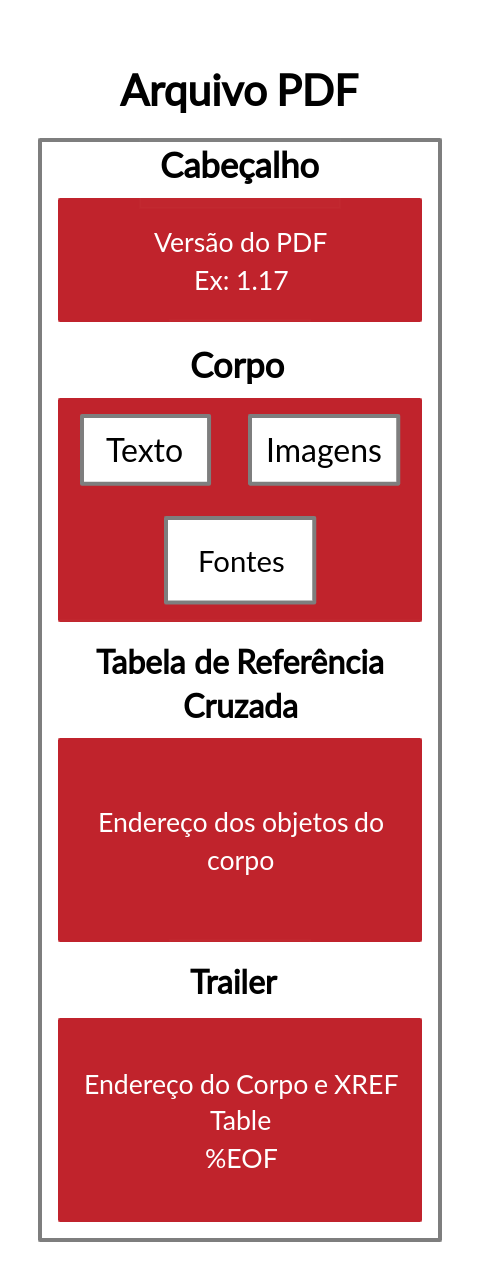
\includegraphics[width=0.3\textwidth]{figs/PDF.png}
\end{figure}

\subsection{Obstáculos na Análise dos Dados}

A extração e análise de dados na área acadêmica é um problema abordado desde a padronização e reconhecimento dos arquivos PDF como um formato universal. O seu crescimento faz com que a análise e extração destes documentos recebam cada vez mais atenção, de diferentes áreas. Como já podem ser encontradas pesquisas que abordam o reconhecimento de fórmulas matemáticas, códigos genéticos, gráficos, entre outras informações. Por ser mais conveniente, são buscadas ferramentas que transformem o arquivo em uma forma intermediária, como por exemplo texto ou HTML, para que seja mais fácil a extração e análise de dados (\citeauthor{ajedig2011pdf}, \citeyear{ajedig2011pdf}).

Com essas abordagens, chegam os desafios, como exemplo, a falta de estrutura padronizada, diferentes formatos dado o software que gerou o arquivo, a incapacidade de renderizar o conteúdo corretamente entre outros. Como foi apresentado no tópico anterior, sabemos que a fonte do PDF não contém as informações de uma forma coerente a leitura humana, e sim blocos que são distribuídos e montados no momento da visualização do arquivo, assim, é necessária realizar uma abordagem na qual as informações buscadas sejam coerentes e não blocos soltos. Outra dificuldade que é muito encontrada está nas diferentes formas que um software pode gerar um arquivo PDF, como no LaTeX, onde certos símbolos matemáticos são desenhados como objetos e no Microsoft Word são utilizados os símbolos Unicode (\citeauthor{sasirekhatext}, \citeyear{sasirekhatext}). A abordagem através do reconhecimento de imagem é muito comum mas enfrenta um grande problema como falsos positivos (\citeauthor{ajedig2011pdf}, \citeyear{ajedig2011pdf}).

Com o objetivo de criar algo mais genérico e reaproveitável para o meio acadêmico, foi pensando em uma forma mais volátil de se realizar a análise dos dados diretamente do PDF montado, e superar as barreiras citadas anteriormente.

\section{Tecnologias}
Como um dos objetivos deste desenvolvimento é criar uma ferramenta que pudesse ser acoplada a outras aplicações e fornecesse a liberdade de ser utilizada em diferentes partes de \textit{front-end}, foi escolhido o formato de API. 

\subsection{API - Interface de Programação de Aplicações}
Uma API é um software intermediário que permite a interação com diferentes aplicações. Ela vai além do que seu nome sugere, e atua principalmente na questão de interface, o grande foco de tal está na forma em que ela se apresenta, isso se tratando de quem a consome, que pode ser tanto para programas quanto para humanos. E se tratando de uma API web, essa interface pode ser acessada em qualquer lugar do mundo. Ela atua recebendo requisições de outra aplicação, então uma rotina correspondente é executada e uma resposta é devolvida a aplicação que realizou a requisição (\citeauthor{designingapioriley}, \citeyear{designingapioriley}).

\begin{enumerate}
  \item REST - Transferência de Estado Representativo
  
  Fielding et al. (\citeyear{fielding2000rest}) propôs em sua tese de doutorado, comparando com estilos arquiteturais já existentes, um estilo para API onde as necessidades de uma aplicação em rede fosse atendidas da melhor forma, e conseguissem que o desenvolvedor seguisse esse padrão sem grandes complicações. Os principais benefícios trazidos pelo REST contam com (\citeauthor{rest2018or}, \citeyear{rest2018or}):
  
  \begin{itemize}
    \item Performance: Resultante de uma comunicação simples e eficiente.
    \item Escalabilidade: Havendo interações simples, é mais prático o crescimento do sistema.
    \item Simplicidade de Interface: Uma interface simples garante uma interação simples e consequentemente traz benefícios como os citados anteriormente.
    \item Manipulação de componentes: Seguindo este estilo há uma separação de responsabilidades, logo um componente não deve depender do outro o que permite que a alteração de um não cause danos a outros.
    \item Portabilidade: Com uma comunicação e Interface simples qualquer API que adote o estilo REST consegue ser consumida por qualquer tipo de tecnologia.
    \item Confiabilidade: Devido a suas restrições, cada requisição é um processo independente o que facilita na recuperação em caso de falhas.
    \item Visibilidade: A Restrição Stateless determina que cada requisição deve ser independente, logo, se forem feitas diversas requisições cada uma deve ter sua resposta e a visibilidade das respostas não precisam ser analisadas.
  \end{itemize}
  
  Fielding et al. (\citeyear{fielding2000rest}) abordou a definição do REST a partir de restrições, elas definem limites e regras para os componentes que compõe o sistema. São seis restrições: 
  
  \begin{enumerate}
    \item Client-Server: É a restrição mais básica, ela garante que a API irá lidar com a comunicação com o banco de dados, gerenciamento de cache, log, etc. Desta forma são separadas as responsabilidades do front-end e do back-end.
    \item Stateless: Como dito anteriormente, esta restrição diz que o cliente pode fazer várias requisições, isso significa que para cada requisição que ele fizer deve ser enviado todas as informações novamente.
    \item Cacheable: Esta restrição não precisa ser aplicados para todos componentes, ela define que a informação de resposta deve ser guardada em cache. No caso de muitas requisições a mesma informação não é necessário ocorrer todo o processo de busca no banco de dados e processar os dados.
    \item Uniform Interface: Tendo uma interface uniforme para todas as requisições o cliente sabe exatamente o formato de resposta que ele deve esperar e é possível ter o mesmo resultado para diferentes plataformas que estiverem consumindo a API.
    \item Layered System: Tendo em mente que que a API está conectada a internet e deve ocorrer um grande tráfego de informação, é aplicado o conceito de camadas para que haja uma simplificação do sistema e uma boa organização dos componentes. Cada camada tem sua responsabilidade, como por exemplo executar a lógica e buscar ou salvar informações.
    \item Code-On-Demand: Única restrição opcional, ela permite que o cliente execute código da lógica do servidor através de um script.
  \end{enumerate}
  
  Estas restrições atuam como paredes invisíveis e conseguem guiar o desenvolvedor. Aplicando estas condições no código é possível obter várias vantagens e construir uma API de ótima performance, coesa e escalável.Quando estas restrições são aplicadas de forma correta no projeto, é utilizada a expressão RESTful para identificar que aquela API está incorporando os limites dado pelo estilo de arquitetura REST.

  \item XML vs JSON
  
  \citeauthor{xml2012} descrevem que o massivo aumento da web trouxe uma grande necessidade de um formato para troca de dados entre diferentes tecnologias. Não havia um formato padronizado de forma que, automaticamente, os dados exportados fossem entendidos ao serem importados em outra aplicação. Com essa necessidade \cite{Sperberg-McQueen:08:EML} junto ao W3C, criaram o XML (\textit{Extended Markup Language}), sendo uma linguagem de marcação, assim como o HTML, mas atendendo a demanda da troca de dados. Atualmente é a forma mais adotada para documentação e registro de dados simples.
  
  Atualmente existem várias alternativas ao XML, sendo as mais famosas JSON e YAML, neste tópico trataremos apenas da comparação com o JSON. O \textit{JavaScript Object Notation} (JSON) é um formato de texto criado para representar um objeto JavaScript, de forma simples, portável e textual (\citeauthor{json2014disponivel}, \citeyear{json2014disponivel}). 
  
  Se tratando uma forma mais compacta, menos verborrágica e com o crescimento do número de aplicações escritas em JavaScript, o JSON se tornou muito popular e vem tomando espaço do XML quando se trata de troca de dados entre plataformas. \citeauthor{xml2012} realizaram uma comparação onde as seguintes vantagens são atribuídas ao JSON.
  
  \begin{itemize}
      \item Velocidade: A análise e leitura de arquivos XML tendem a ser lentas, devido a sua verborragia, enquanto o JSON entrega os dados de forma simples e direta.
      
     \item Serialização e Desserialização: Normalmente é encontrada uma única forma, e já presente no JavaScript, para a transformação dos dados de JSON para bytes, e vise-versa.
     
     \item Conciso: O JSON utiliza a técnica de chave-valor, enquanto o XML utiliza tags, o que dificulta a visualização e aumento o tamanho do arquivo.
     
     \item Bibliotecas de fácil utilização: Atualmente é possível encontrar bibliotecas, para a maioria das linguagens, que tornam a utilização do JSON muito orgânica, enquanto a utilização do XML é algo mais complicado.
  \end{itemize}
  
  Dado as vantagens, e a escolha do Node.js, que será melhor abordada no próximo tópico, foi decidido que todos os dados na aplicação serão trabalhados no formato JSON.
  
  \item \textit{Middleware}
  
  
  
\subsection{Node.JS}

Node é a forma de utilizar JavaScript em um servidor. A implementação do Node tem base no interpretador JavaScript desenvolvido pela Google, o V8, este interpretador é implementado em C e C++, e se concentra em extrair a melhor performance utilizando menos memória (\citeauthor{tilkov2010node}, \citeyear{tilkov2010node}). 

Motivado a criar uma comunicação simples entre o servidor e a página web, Ryan Dahl criou o Node.js em 2009 e foi um sucesso imediato. Fundamentado em ser Event Driven, o que quer dizer que há sempre um core escutando por todos os eventos, e chamando as devidas funções quando tais eventos são acionados; somado com o JavaScript foi obtido um web server rápido e acessível a toda comunidade web que já tinha familiaridade com a linguagem, o que foi essencial para que o Node fosse tão amplamente adotado (\citeauthor{shah2017node}, \citeyear{shah2017node}).

A introdução do Node trouxe características de outras linguagens que não existem no JavaScript no navegador, como a manipulação do sistema de arquivos, acesso a um banco de dados e a criação de um cliente HTTP, o que faz possível a criação de um web server  (\citeauthor{mead2018learning}, \citeyear{mead2018learning}). Pela familiaridade de grande parte dos desenvolvedores web com a linguagem JavaScript e a crescente onde de separação de Front-End e Back-End, a criação de API's utilizando o Node.JS se tornou muito popular e atualmente, boa parte das ferramentas encontradas para atingir os objetivos deste trabalho podem ser encontradas como bibliotecas de tal.

\begin{enumerate}
    \item NPM - \textit{Node Package Manager}
    No mesmo ano de lançamento do Node.JS foi lançado o \textit{Node Package Manager} (NPM), que atua como um gerenciador e distribuidor de pacotes para projetos, e conta com uma interface por linha de comando que auxilia na criação e manejo de tais. 
    Atualmente o NPM é o maior registrador de software do mundo, devido a sua facilidade e a imensa comunidade dos usuários. 
    Em poucos segundos é possível submeter um pacote ao NPM e assim com a visibilidade e apoio da comunidade este pacote é mantido e utilizado livremente por desenvolvedores ao redor do mundo. Muitas tarefas específicas e morosas são evitadas através da utilização de algum pacote que já contém determinada solução para tal tarefa.
    Uma importante tarefa que o mesmo executa é o controle de versão de dependências, isto é, um pacote pode utilizar determinada versão de outro, e através de um arquivo chamado \textit{lockfile} é obtida determinada versão da dependência de forma que o pacote não encontre problemas de outras versões da dependência. A utilização do NPM em projetos Node é algo indispensável e de grande utilidade. Desta forma, este foi utilizado para o controle de bibliotecas e organização do projeto (\citeauthor{npm}, \citeyear{npm}).

\end{enumerate}

\subsection{NoSQL}

Estabelecido que o sistema terá como base uma API em Node.JS, foi necessário escolher um banco de dados. Pensando na melhor integração com o Node.JS, a possibilidade de escalar para uma massiva quantidade de dados e a compatibilidade com chave-valor proveniente dos objetos JSON; foi feita uma análise dos bancos NoSQL.

O NoSQL é uma categoria de banco de dados que surgiu com o objetivo de atender aos requisitos do gerenciamento de grande volume de dados, sem estrutura definida e que necessitam ser disponibilizados rapidamente e preparados para crescer ainda mais. Esta categoria traz algumas características como: (\citeauthor{loscio2011nosql}, \citeyear{loscio2011nosql}).

\begin{itemize}
    \item Evitamento de Complexidade desnecessária.
    \item Alta Taxa de Transferência: A maioria dos bancos não relacionais conseguem ter uma boa vantagem na taxa de transferência quando comparados aos relacionais.
    \item Escalabilidade Horizontal.
    \item Esquema Flexível ou Ausência de Esquema: A ausência ou flexibilidade de esquema trás vantagens como a alta escalabilidade e a oportunidade de mudar ou adicionar campos inesperados. Há a desvantagem da falta de garantia de integridade dos dados.
    \item Simples Acesso aos Dados: Com o foco em velocidade é essencial que a entrega de dados ao sistema seja feita de forma simples e enxuta, o modelo NoSQL oferece os dados como interface e facilita o acesso e utilização de tal.
    \item Modelo Chave-Valor: O modelo simples torna prático o armazenamento de dados, principalmente quando se trata de algo que não necessita se relacionar com outros valores e independe do tamanho do valor.
\end{itemize}
  
\section{Estado da Arte}  

Se tratando de outros programas que em sua essência realizam a análise extração de dados foram encontradas boas alternativas, mas nenhuma que contemplasse todos os objetivos que foram postos aqui. A seguir serão apresentadas essas alternativas e definido porque ela não se encaixa no objetivo deste projeto.

\begin{itemize}
    \item \cite{pdft}, \cite{fpdfc} e \cite{tabula} São boas alternativas, grátis mas que realizam apenas a extração de dados tabulares e geram arquivos \textit{.csv}. Não satisfazendo os quesitos de ser genérico e ter a capacidade de se acoplar a outra aplicação.
    
    \item \cite{lapdf} é uma alternativa desenvolvida por biomédicos que buscavam extrair dados de artigos, ela ainda está em desenvolvimento, porém o foco dela é a extração de dados somente de artigos. Assim, ela está engessada ao layout de artigos e não funciona com outros tipos de arquivo. Apresenta as mesmas incapacidades das alternativas anteriores, quanto aos objetivos deste projeto.
    
    \item \cite{epdf} é uma alternativa online e grátis que realiza a conversão do PDF em arquivos de texto e imagens. Em testes feitos neste site, foi notado que a extração de texto é feita em blocos quebrados que nem sempre estão na ordem correta de leitura. Não torna possível a utilização em outras aplicações e não possibilita a seleção de quais dados serão extraídos.
    
    \item \cite{dparser} apesar de ser uma alternativa paga, pelo que foi apresentado realiza a extração dos dados dada as coordenadas e página, resultando em um arquivo de texto com os dados extraídos. 
    
    \item \cite{ipdf} Uma ótima alternativa que pode ser utilizada com aplicações em Java e C++, possui uma API e uma interface amigável caso necessário, e diversos modos de configuração para que se atinja a extração do dado necessário. Porém é uma alternativa paga.
    
\end{itemize}

\end{enumerate}
\chapter{Materiais e Métodos}

Esta seção descreve as etapas do desenvolvimento da API, assim como a aplicação e utilização das ferramentas e suas tecnologias. Este desenvolvimento foi realizado utilizando a generalização de conceitos de engenharia de software, com o objetivo de gerar desacoplamento e reutilização de código. As etapas de desenvolvimento se deram através das etapas necessárias para a construção de uma API REST e organizadas utilizando a metodologia ágil Kanban.

\section{Bibliotecas e Ferramentas}

A escolha das bibliotecas e softwares deste projeto, devem-se a pesquisas que tiveram como foco: 
\begin{itemize}
    \item Suporte dos desenvolvedores: Dada a necessidade de se ter uma ferramenta que seja confiável e atualizada.
    \item Alta utilização pela comunidade: Já que a maioria destas ferramentas são de código livre e podendo a comunidade submeter melhorias e realizar fiscalização do que está sendo alterado na mesma.
    \item Compatibilidade a outros componentes e estrutura do projeto: Um dos objetivos deste software é que ele seja mutável, para que de acordo com as mudanças que podem ocorrer em outras tecnologias e estruturas de documentos PDF, esteja apto a acompanhar tais alterações.
\end{itemize}

\subsection{PDF.JS - v2.2.228}

O PDF.JS, criado em 2011 pela Mozilla Foundation, é uma biblioteca amplamente utilizada, e se encontra presente na maioria dos websites que fazem qualquer tipo de manipulação e exibição de PDF. Esta foi criada como uma extensão do navegador Firefox, com a intenção de renderizar arquivos PDF, de forma rápida e segura, no navegador do cliente. Apesar da migração de uma biblioteca específica para o navegador da Mozilla, seu formato de renderização permanece o mesmo, onde ela acessa a estrutura do arquivo PDF, coleta o conteúdo e a formatação no \textit{Body}, realiza a conversão para HTML e CSS de cada objeto encontrado e com a tabela XREF o arquivo é remontado no navegador do cliente como um PDF dentro da página.

Com a evolução das tecnologias e a busca contínua por melhor performance, esta biblioteca conta com centenas de funções e diferentes abordagens para e leitura das mais variadas formas de PDF. Utilizando o resultado destas funções, é possível realizar extrações para coleta de informações encontradas no arquivo, informações como o texto puro, posição de elementos na página, fonte utilizada, cor e vários outros tipos.

Como o objetivo deste sistema está diretamente ligado a extração dos dados e o foco principal desta biblioteca é a renderização do arquivo no navegador, boa parte das funções mais pesadas nesta biblioteca não são necessárias.

\subsection{Extract - v0.1.3}
Convenientemente, há um módulo criado pela comunidade que encapsula somente a parte e extração de dados contida na biblioteca e entrega de forma leve e prática todas as funcionalidades necessárias para uma boa extração do conteúdo do arquivo PDF.

Fundamentalmente, a leitura acontece de forma que, dado o caminho do arquivo e um objeto de opções, onde podem ser especificadas quais páginas deve ser lidas, a formatação dos espaços entre outro, são extraídos metadados do arquivo como o autor, o software utilizado para salvar o arquivo, o software utilizado para gerar o PDF, última data de edição entre outros. Junto ao objeto de metadados é retornado um vetor contendo um objeto JSON para cada página analisada, este objeto contém todas as informações básicas necessária para análise do conteúdo como é possível ver  \textbf{Figura \ref{pdfExtract}}

\begin{figure}
\centering
\captionsetup{justification   = raggedright,
              singlelinecheck = false}
\caption{Objeto JSON após extração de informação de um PDF através da biblioteca Extract}\label{pdfExtract}
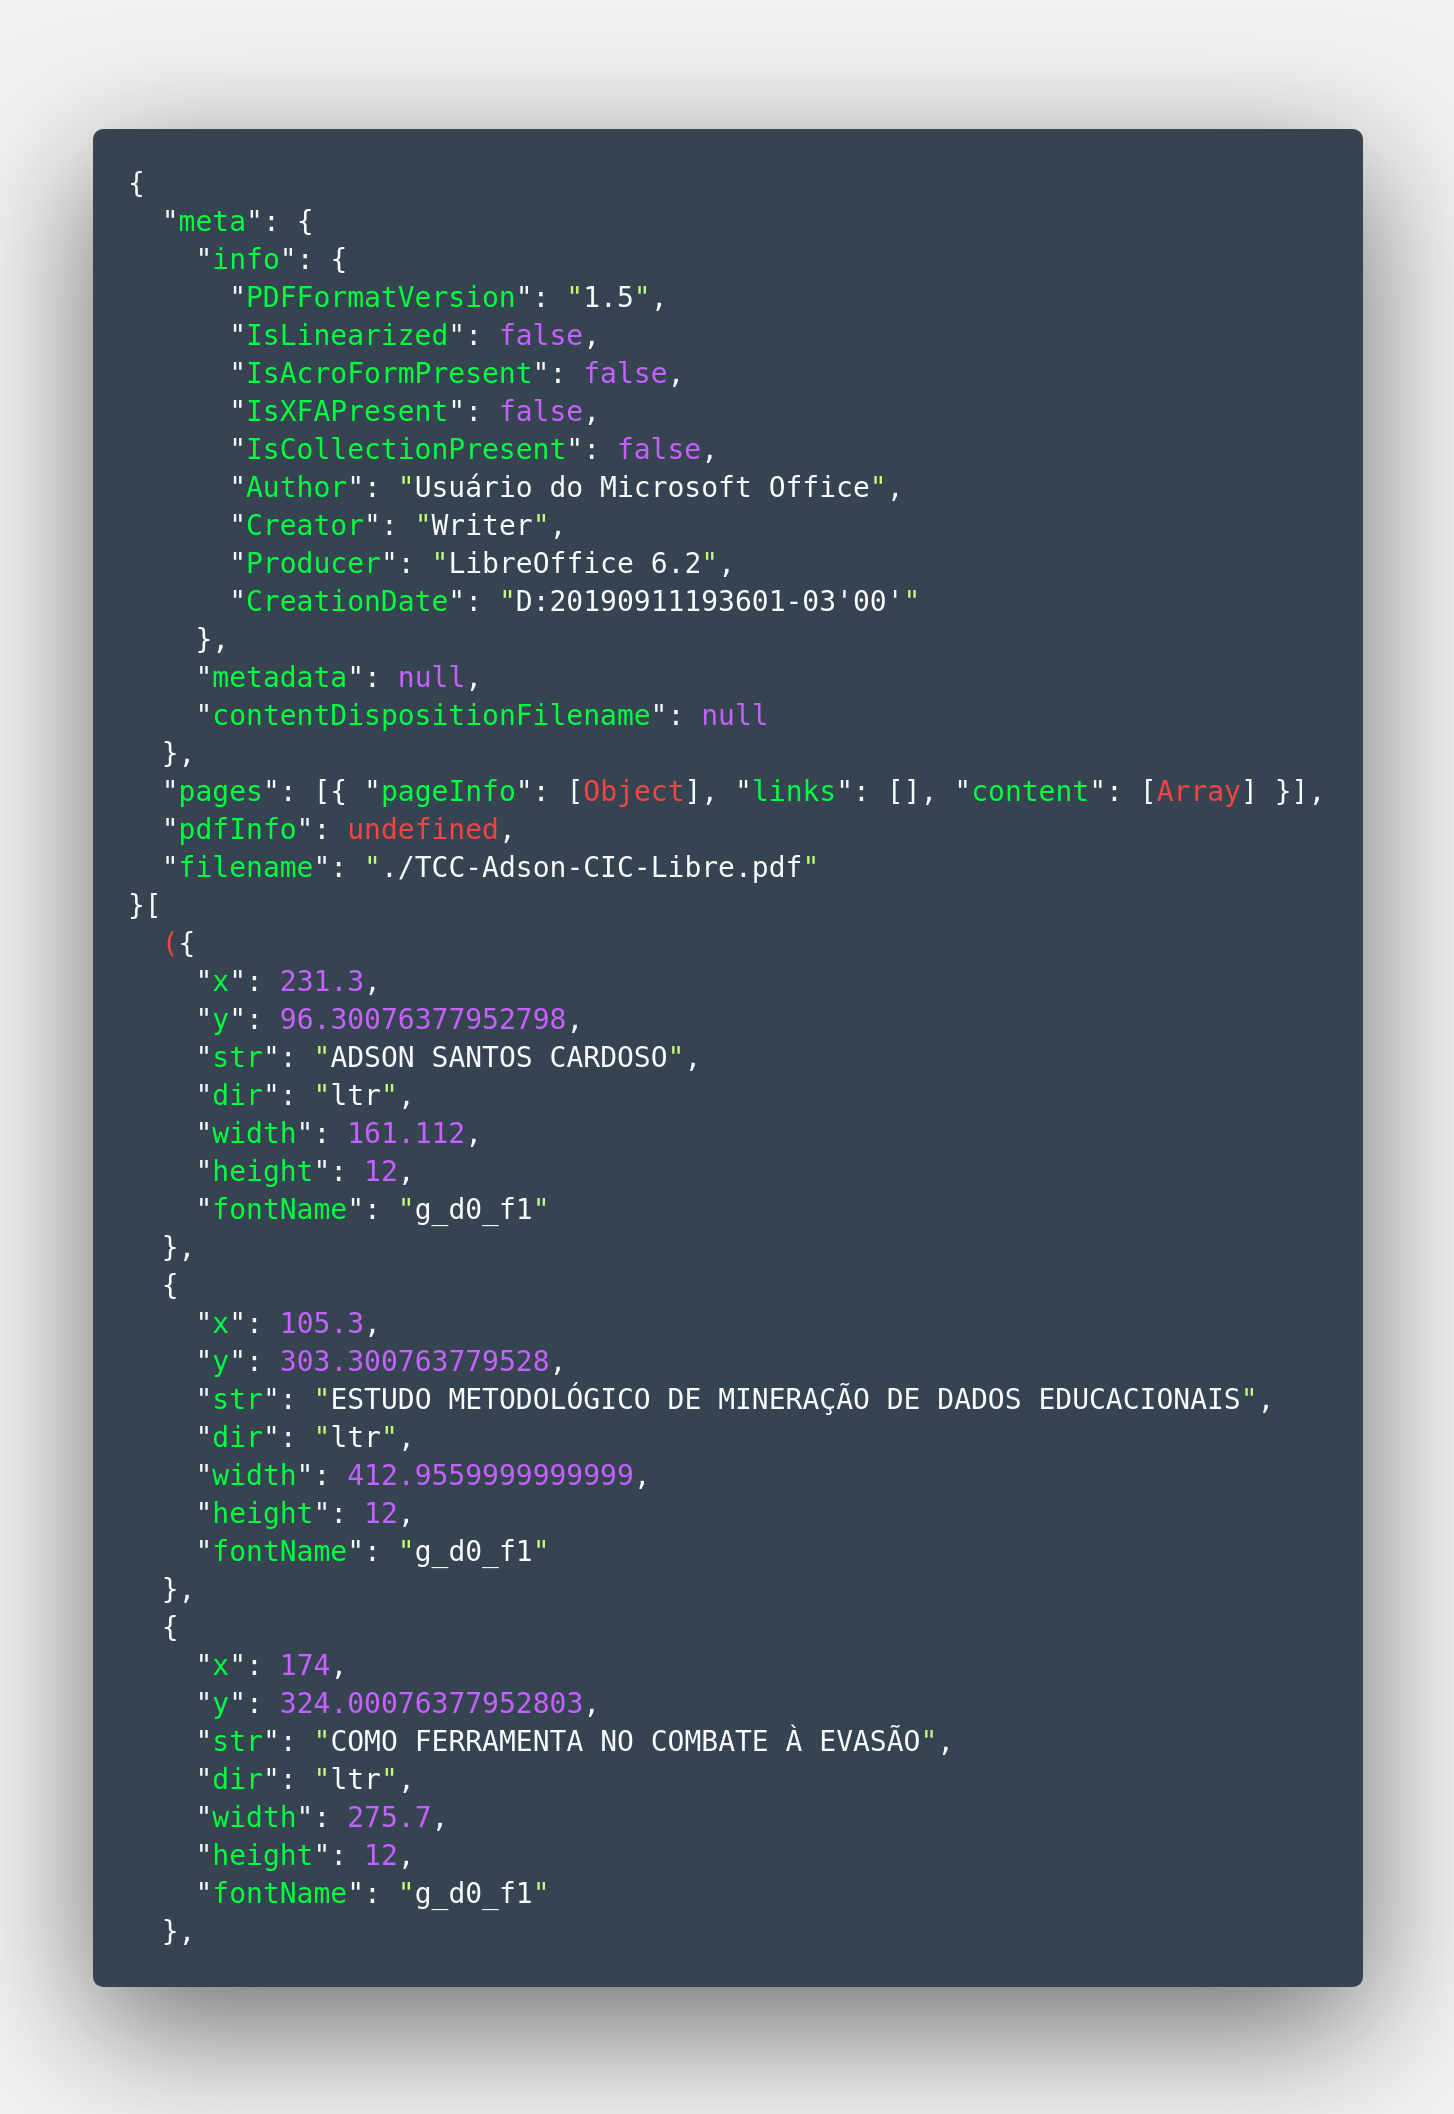
\includegraphics[width=0.8\textwidth]{figs/pdfExtract.png}
\end{figure}

Após extrair essas informações o próximo passo foi a filtragem deste conteúdo.

\subsection{Extract By Coord}

Dado o objetivo de extrair a informação dado um espaço da página, definido por coordenadas X e Y, foi feita uma pesquisa de formas práticas para se realizar a filtragem do conteúdo, por tais coordenadas, assim foi encontrada uma pequena biblioteca no GitHub, com a licença MIT, que realizava uma abordagem similar a necessária para a próxima etapa da extração dos dados.

Esta biblioteca oferece duas funcionalidades, a primeira encapsula a extração feita pela biblioteca Extract, com o intuito de descartar informações desnecessárias para a análise, como a rotação, escala, tamanho da página, e evidenciar o software responsável por gerar o arquivo PDF, a importância desta informação será detalhada no tópico X. Além disso, os objetos na página são ordenados da esquerda a direita e de cima para baixo, e selecionado apenas os dados de coordenadas e string. Desta forma é retornado um objeto JSON enxuto, contendo apenas as informações necessárias e pronto para ser recebido como entrada da segunda função. 

Esta função é responsável por extrair o conteúdo, ela recebe o nome do programa responsável por gerar o arquivo PDF, a importância deste valor é decorrente da forma que diferentes programas atribuem diferentes formas de espaçamento entre as strings, por exemplo o Microsoft Word realiza o espaçamento dos objetos atribuindo vários objetos de espaço, além disso são recebidos o objeto da página a ser extraída, e as coordenadas X e Y de início e de fim como objeto JSON. Ao ser executada, são observadas as coordenadas de cada objeto dentro da página, estando no alcance das coordenadas recebidas, sua string é extraída e tratada, de acordo com o software que gerou o arquivo PDF. Desta forma é retornada uma string com o que se encontra naquela região.

Esta biblioteca foi alterada para que o texto recebido fosse entregue com uma formatação correta, devido a diferença de espaços causada pelo software que gerou o PDF, além disso foi feita uma melhor filtragem pelo sistema de coordenadas e a função de extração passou a aceitar mais de uma página.

\subsection{RegEx - Expressão Regular}
O RegEx, derivado da expressão regular definida na teoria da computação, entrega uma forma de se identificar cadeia de caracteres, dada uma expressão regular em linguagem formal. Ou seja, dada uma expressão é possível encontrar cadeias que aceitem tais condições. A linguagem JavaScript carrega todo um grupo de funções que auxiliam na utilização de expressões regulares, assim não é necessária nenhuma biblioteca adicional.

Como forma de limitação ou busca de valor específico são utilizadas expressões regulares que tanto removem trechos que podem afetar a busca de um valor, quanto encontram um valor específico após determinada palavra. Como por exemplo no caso de haver um Coorientador quando se está um busca do nome do Orientador, então é feita a busca pelo Coorientador e se encontrado seu valor é retirado, isso ocorre devido a utilização da expressão regular com \textit{lookbehind}(olhar atrás), já que o valor buscado está depois da palavra Orientador, então retirar o Coorientador serve como uma condição de parada, assim como pontuação e quebra de linha.

A filtragem com o RegEx assegura o conteúdo encontrado e delimita a informação buscada, no caso de ocorrer um bloco inesperado dentro das coordenadas. 

\subsection{JWT - \textit{JSON Web Token} (v8.5.1) }

Com a necessidade de se ter uma forma de autenticação segura e prática, foi optado pela utilização do \textit{JSON Web Token}. Comumente, o desenvolvedor realiza a implementação de seu próprio método de autenticação, porém, segundo a \textit{Open Web Application Security Project} (OWASP), uma organização sem fins lucrativos que trabalha em prol da segurança na web, buscando falhas e formas de combater as mesmas, a “Quebra de Autenticação e Gerenciamento de Sessão” é um dos maiores e mais recorrentes problemas em aplicações web. A falta de uma boa criptografia e métodos seguros de envio e recebimento de dados ocasiona oportunidades para que usuários mal intencionados consigam invadir contas e ter acesso a informações sigilosas.

O JWT é um padrão aberto (RFC 7519), que define de forma compacta, independente e segura, um método de transmitir informações como objeto JSON. Sendo uma forma segura, com bibliotecas para a maioria das linguagens utilizadas na web e suporte nativo do JSON nos navegadores modernos,  o JWT se tornou a escolha ideal como método de autenticação. 

Utilizando o algoritmo HMAC \textit{(Hash based Message Authentication Code)}, a informação é encriptada com um segredo que apenas o lado do servidor contém, (também podem ser utilizados pares de chaves pública/privada através da encriptação por RSA ou ECDSA), e passada como um cabeçalho HTTP. Desta forma, quando o usuário realiza uma requisição, o servidor chama um método de validação do \textit{token} (\cite{jwt}).

\subsection{MongoDB}

O MongoDB é um banco de dados não relacional, onde os dados são armazenados em documentos JSON, por isso é dito que este é um banco orientado a documentos. Desta forma não há necessidade da criação de tabelas e colunas na fase de modelagem do banco, assim há uma liberdade maior para que o documento que será salvo represente apenas as informações necessárias e suas relações não sejam pré definidas.

Esta flexibilidade é de grande ajuda quando se trata de uma aplicação que pode mudar a organização e o tipo de informação a ser salva, diferente de um banco relacional, onde toda sua estrutura deveria ser mudada para que se adequasse a estas mudanças. No caso dessa aplicação, o usuário irá definir quais informações serão extraídas do PDF e assim o objeto JSON com as informações será montado, além disso o usuário também tem a liberdade de adicionar ou remover um campo de informação a ser extraída ou adicionar um novo sem afetar a estrutura do banco.

A escolha do MongoDB entre os bancos não relacionais foi feita devido a sua alta performance, facilidade de manipulação em relação a sua infraestrutura, popularidade e principalmente a biblioteca Mongoose. 

\subsubsection{Mongoose}

O manipulação do Mongo foi feita através da biblioteca Mongoose, onde a modelagem de dados é baseada em esquemas. Ao realizar uma consulta ao banco de dados, através do mongoose, é realizada conversão do dado para um objeto JavaScript, assim quando recuperada uma informação do banco, sua manipulação se torna algo simples e orgânico no fluxo de desenvolvimento. Também é possível realizar validações através da declaração do esquemas, isso impõe mais uma camada de segurança entre o usuário e a API. 

\section{Metodologia e Desenvolvimento}

Neste tópico, serão explicados como cada ferramenta, definida no tópico anterior foi utilizada. Os detalhes mais específicos podem ser encontrados no repositório deste projeto no GitHub, publicamente aberto e é possível enviar mudanças para que sejam avaliadas e incorporadas no código. Também será descrito como foi modelada a estrutura deste sistema e dividia as etapas de desenvolvimento.

\subsection{Metodologia Ágil}

Para a organização e definição das tarefas que objetivam a completude deste projeto foi escolhida a metodologia ágil Kaban. Criado pela Toyota nos anos 70, o Kanban (que pode ser traduzido como Cartão),  sinalizava a disponibilidade para se trabalhar em uma peça, quando se fazia necessário para outras etapas da produção. Dessa forma havia uma maior organização na ordem de trabalho, não havia desperdício de peças e através dos cartões era possível ver o progresso geral.

Com estas vantagens é possível aplicar ao desenvolvimento de software o Kanban e trazer até mais algumas vantagens ao fluxo de trabalho para a programação. 
Aplicando esta metodologia é feito um quadro consistente de três colunas, uma de tarefas \textbf{A fazer}, em seguida as tarefas \textbf{Em andamento} e finalizando com as tarefas \textbf{Concluídas}.

O GitHub oferece uma implementação do Kanban, diretamente no repositório para que outros colaboradores possam interagir e a visualização e utilização sejam práticas.

Foram separados por ordem de prioridade as tarefas necessárias para atingir a completude da API, e adicionadas nas lista de A fazer no kanban, foram priorizadas aquelas que eram necessárias para o funcionamento e teste da API, assim foi feito uma por vez até que houvessem mais tarefas que impedissem o funcionamento de tal.

\subsection{MVC - \textit{Model View Controller}}

A estrutura deste sistema foi elaborada de acordo com o padrão de desenvolvimento MVC,
\chapter{Resultados} \label{resultados}

A API pode ser encontrada em funcionamento em um ambiente de testes no link \href{http://bit.ly/tcc-pdf}{http://bit.ly/tcc-pdf}. Suas funcionalidades de leitura encontram-se livres para serem acessadas, porém as funcionalidades que alterem o estado do banco de dados estão restritas aos usuários cadastrados. Apesar de estar em funcionamento e livre para ser acessada, este é apenas um ambiente de testes, e sua hospedagem no servidor do Núcleo de Biologia Computacional e Gestão de Informações Biotecnológicas (NBCGIB) está sendo configurada.

Para o controle destas utilidades existem duas camadas de segurança. 
A camada de chave de API, apresentada na \textbf{Figura \ref{swaggerAPIKey}} assegura que somente os administradores do sistema, em posse da chave, possam registrar e remover usuários da API.

\begin{figure}[H]
\centering
\captionsetup{justification   = raggedright,
              singlelinecheck = false}
\caption{Autorização por Chave de API - Swagger UI}\label{swaggerAPIKey}
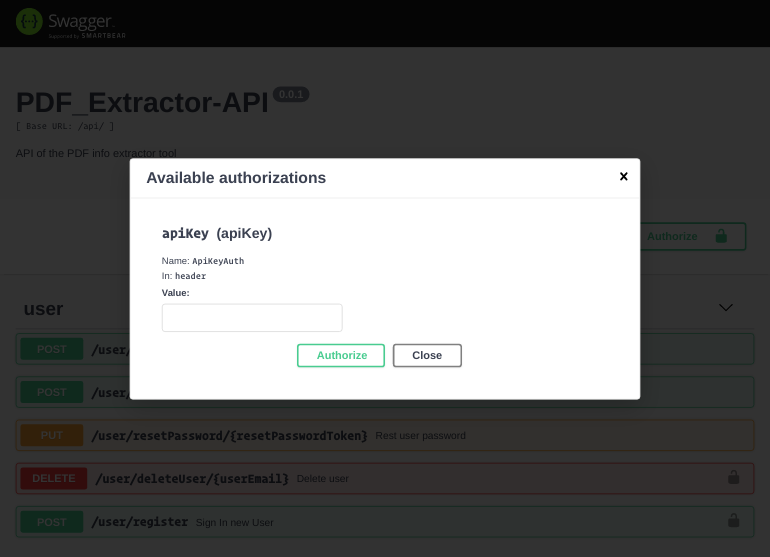
\includegraphics[width=0.9\textwidth]{figs/swaggerAPIKey.png}
\footnotesize Fonte: Autoria Própria
\end{figure}

A camada de usuário garante a integridade do sistema, pois esta impede que usuários não autenticados tenham acesso a funcionalidades que alterem o estado do banco de dados. Na \textbf{Figura \ref{swaggerLogin}} é possível ver o método de login, e suas possíveis respostas.

\begin{figure}[H]
\centering
\captionsetup{justification   = raggedright,
              singlelinecheck = false}
\caption{Login de Usuário - Swagger UI}\label{swaggerLogin}
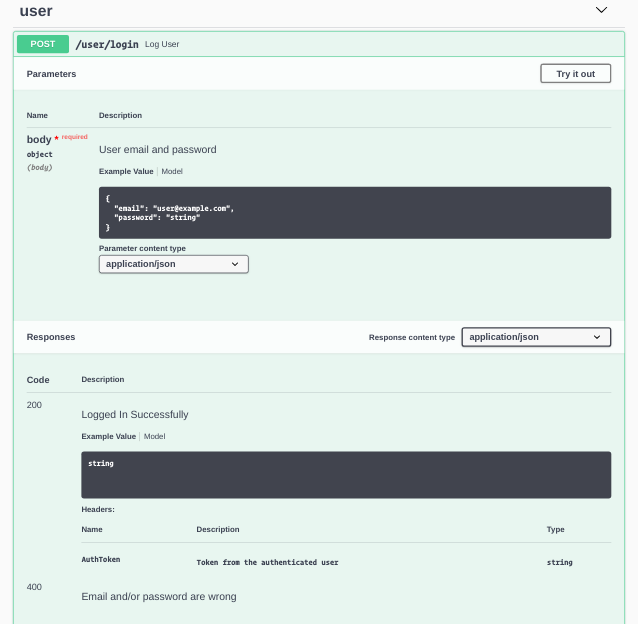
\includegraphics[width=1\textwidth]{figs/swaggerLogin.png}
\footnotesize Fonte: Autoria Própria
\end{figure}

Para o categoria de funções do usuário, assegurando o acesso e contendo funcionalidades necessárias para o administrador do sistema apresenta as seguintes funcionalidades:

\begin{itemize}
    \item \textbf{Login}: Como explicado no tópico \ref{apiDev}, recebe e-mail e senha e retorna um \textit{token} caso a autenticação o ocorra com sucesso.
    
    \item \textbf{Senha Esquecida}: Recebe o e-mail do usuário, sendo ele valido, é disparado um e-mail contendo um identificador único para a recuperação da senha.
    
    \item \textbf{Resetar Senha}: Continuando o fluxo da função anterior, recebe o identificador e uma nova senha, caso sejam válidos, a nova senha é atribuída ao usuário.
    
    \item \textbf{Remover Usuário}: Recebe um e-mail de usuário e a chave de API, caso sejam válidos, o usuário correspondente a aquele e-mail é desativado.
    
    \item \textbf{Registrar Usuário}: Recebe e-mail e senha do usuário a ser cadastrado. Também deve ser enviada a chave de API para validação do administrador. A coleção de usuários, no banco de dados, se encontra livre de \textit{schema} devido aos diferentes tipos de usuários. 
\end{itemize}

Para que o usuário tenha controle das configurações do conteúdo a ser extraído, foi criada a seção de Extração:

\begin{itemize}
    \item \textbf{Registrar Parâmetros}: Conforme explicado anteriormente no tópico \ref{apiDev}, esta requisição recebe um objeto JSON, com as informações necessárias para realizar um extração, e o \textit{token} de usuário, como pode ser observado na \textbf{Figura \ref{swaggerExtractParam}}. Este objeto é salvo no banco de dados e utilizado ao realizar extrações.
    
    \item \textbf{Parâmetros Registrados}: Realiza uma consulta no banco de dados e retorna um objeto JSON com um vetor de parâmetros que já estão registrados.
    
    \item \textbf{Remover Parâmetro}: Recebe um ID de parâmetro e o \textit{token} de usuário, sendo válidos, o parâmetro é removido do banco de dados.
\end{itemize}

\begin{figure}[H]
\centering
\captionsetup{justification   = raggedright,
              singlelinecheck = false}
\caption{Parâmetros de Extração - Swagger UI}\label{swaggerExtractParam}
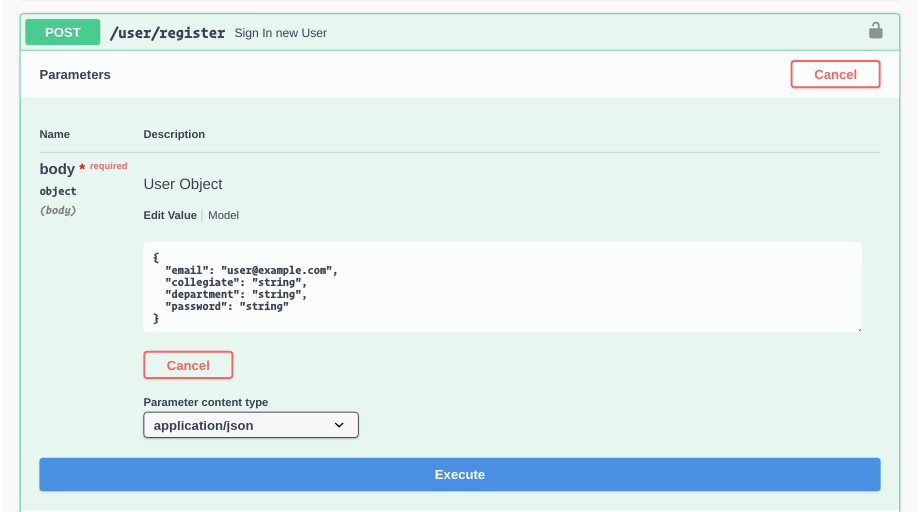
\includegraphics[width=1\textwidth]{figs/SwaggerUIExample.png}
\footnotesize Fonte: Autoria Própria
\end{figure}

Em relação a informação já extraída, são entregues as seguintes funcionalidades:

\begin{itemize}
    \item \textbf{Informações Extraídas}: Consulta no banco de dados todas as informações extraídas e as retorna em um vetor de objetos JSON correspondente a cada arquivo, contendo as informações que foram extraídas de tal.
    
    \item \textbf{Remover Informação Extraída}: Recebe o ID correspondente a um objeto de informações extraídas, e um \textit{token} de usuário, sendo válido, remove o objeto do banco de dados.
\end{itemize}

Por fim há a função responsável por receber um arquivo, o \textit{token} de usuário e a identificação do arquivo, como pode ser visto na \textbf{Figura \ref{swaggerUploadFile}}. Ao ser recebido, são buscados os parâmetros que possuem o mesmo valor do arquivo enviado no campo \textit{docType}, e assim serão extraídas as informações para cada parâmetro definido. A requisição é respondida com um objeto JSON contendo todas as informações extraídas, em caso de sucesso.

\begin{figure}[H]
\centering
\captionsetup{justification   = raggedright,
              singlelinecheck = false}
\caption{Envio de Arquivo - Swagger UI}\label{swaggerUploadFile}
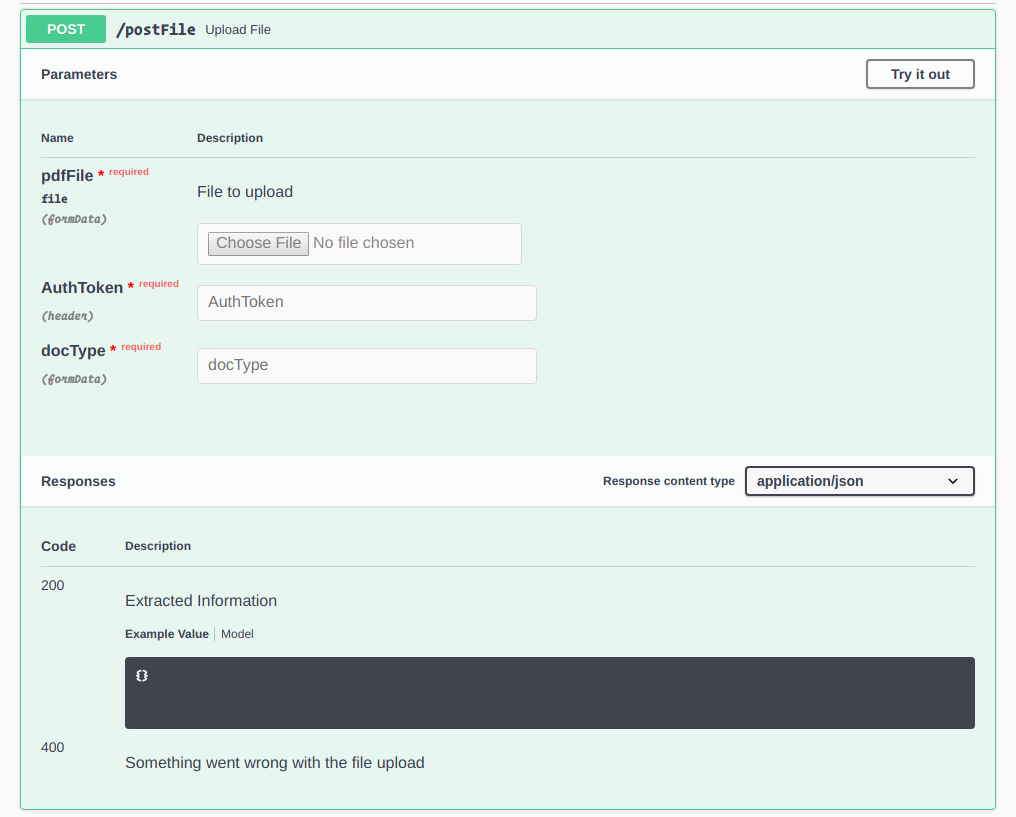
\includegraphics[width=1\textwidth]{figs/swaggerUploadFile.png}
\footnotesize Fonte: Autoria Própria
\end{figure}

Como pode ser notado nas imagens apresentadas neste capitulo, toda a API está documentada e pronta para uso na interface do Swagger, que pode ser encontrada no caminho \textit{/api/docs} (partindo do endereço raiz da aplicação). Neste endereço é possível fazer a utilização da API e ter o entendimento do que cada função faz e o que deve ser retornado.

No curso de Ciência da Computação da UESC há um projeto em desenvolvimento para a criação de uma rede de egressos. Sendo o trabalho de conclusão de curso aprovado, este é o primeiro passo para o aluno se tornar um egresso. Desta forma foi notado que há uma demanda por informações referentes aos egressos que podem ser encontradas no arquivo PDF do trabalho, assim é possível extrair um espécie de ficha do egresso contendo nome do autor, orientador, título do trabalho, palavras-chave e resumo.

Com esta demanda e a necessidade de por a prova a API, foi desenvolvida uma aplicação \textit{front-end} para a utilização do colegiado do curso. 

% Conforme apresentado na figura 12, todas as funcionalidades de usuário da API estão apresentadas nesta tela login

% Conforme apresentado na \textbf{Figura \ref{login}}, todas as funcionalidades, pertinentes a usuário, estão ligadas as funções da API. Esta tela representa a página de login por onde o colegiado deve acessar o sistema.

% Utilizando a chave de API foi criada uma conta de usuário para o colegiado. Na \textbf{Figura \ref{login}} a tela de login no sistema do colegiado é apresentada. Todas as funcionalidades de usuário estão em comunicação com as funções da API.

% \begin{figure}[H]
% \centering
% \captionsetup{justification   = raggedright,
%               singlelinecheck = false}
% \caption{Login - Sistema de Extração de dados de TCC}\label{login}
% 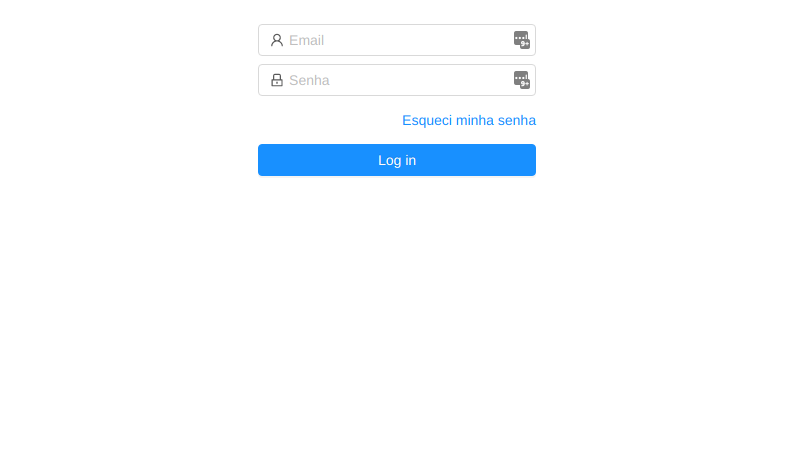
\includegraphics[width=1\textwidth]{figs/tccExtract/login.png}
% \footnotesize Fonte: Autoria Própria
% \end{figure}

Ao acessar a aplicação a tela de login é apresentada, e todas as funcionalidades de usuário da API estão conectadas a tal. Esta tela representa por onde o colegiado deve acessar o sistema.

Após efetuar o login, o usuário deve cadastrar os parâmetros de extração. Como pode ser visto na \textbf{Figura \ref{params}}, é apresentada a tela para cadastro de parâmetros em página específica, e na \textbf{Figura \ref{params2}} para parâmetros de página indefinida. Ao enviar o formulário, o objeto JSON é montado e a RegEx codificada para base64 e assim o cadastro é realizado. Como resultado das informações preenchidas na \textbf{Figura \ref{params}} é apresentado o objeto JSON da \textbf{Figura \ref{jsonParams}}.

\begin{figure}[H]
  \centering
  \caption{Registro de Parâmetro - Sistema de Extração de dados de TCC}
  \subfloat[Registro de Parâmetro de Página Específica]{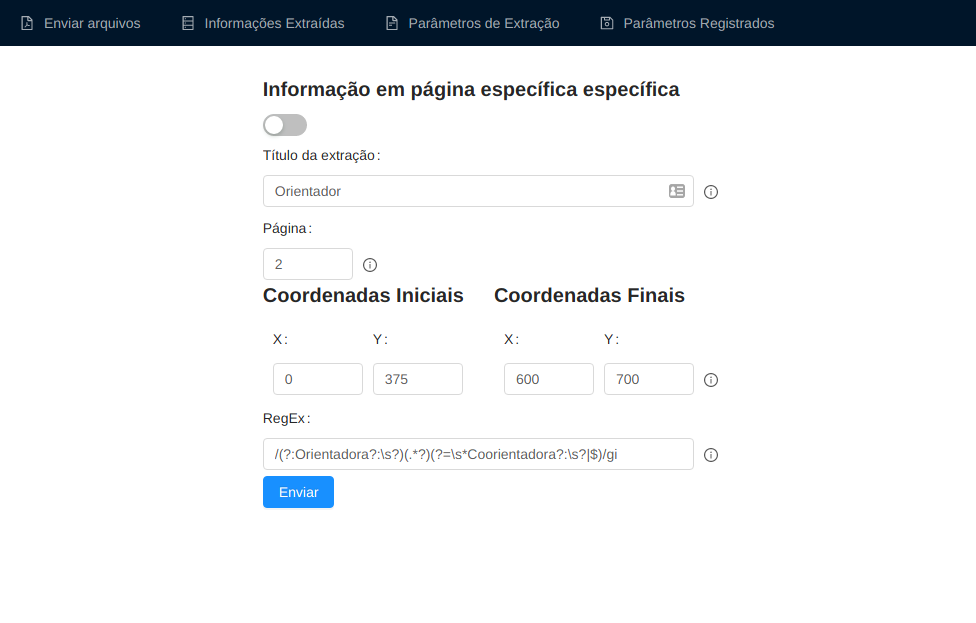
\includegraphics[width=\textwidth]{figs/tccExtract/params.png}\label{params}}
  \hfill
  \subfloat[Registro de Parâmetro de Página Indefinida]{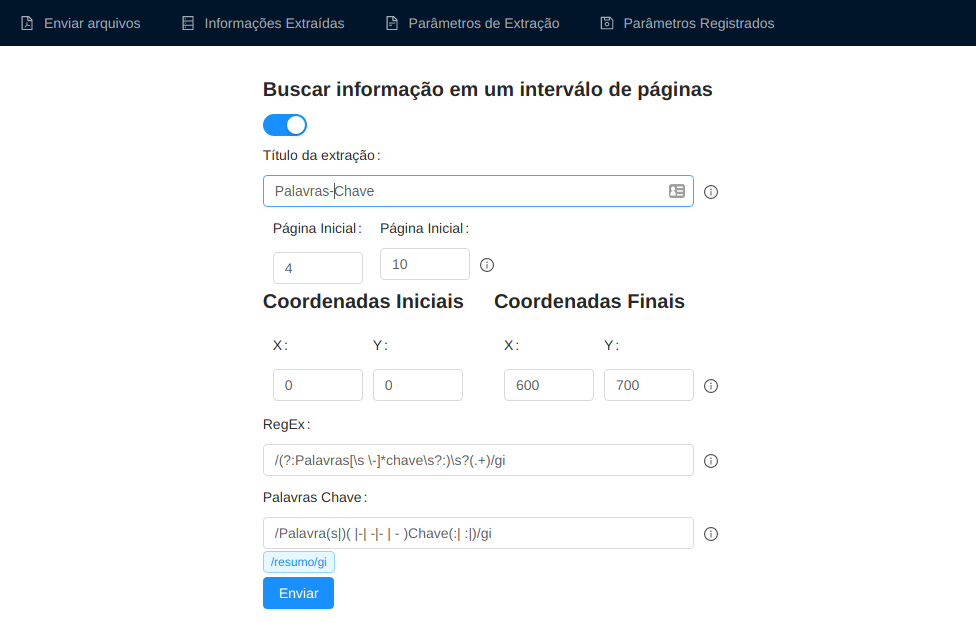
\includegraphics[width=\textwidth]{figs/tccExtract/params2.png}\label{params2}}

\end{figure}

\begin{figure}[H]
\centering
\captionsetup{justification   = raggedright,
              singlelinecheck = false}
\caption{Objeto JSON Resultante do Formulário de Parâmetros de Extração - Sistema de Extração de dados de TCC}\label{jsonParams}
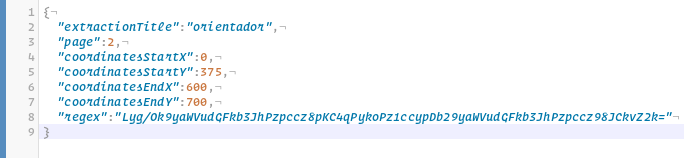
\includegraphics[width=1\textwidth]{figs/jsonParams.png}
\footnotesize Fonte: Autoria Própria
\end{figure}

% \begin{figure}[H]
% \centering
% \captionsetup{justification   = raggedright,
%               singlelinecheck = false}
% \caption{Registro de Parâmetro de Página Específica - Sistema de Extração de dados de TCC}\label{params}
% 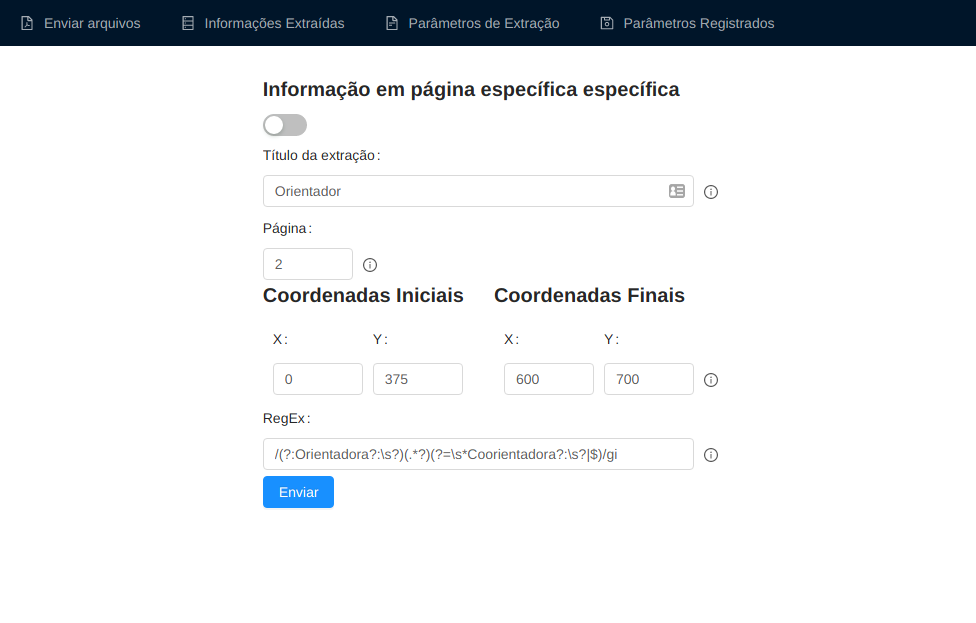
\includegraphics[width=1\textwidth]{figs/tccExtract/params.png}
% \footnotesize Fonte: Autoria Própria
% \end{figure}

% \begin{figure}[H]
% \centering
% \captionsetup{justification   = raggedright,
%               singlelinecheck = false}
% \caption{Registro de Parâmetro de Página Indefinida - Sistema de Extração de dados de TCC}\label{params2}
% 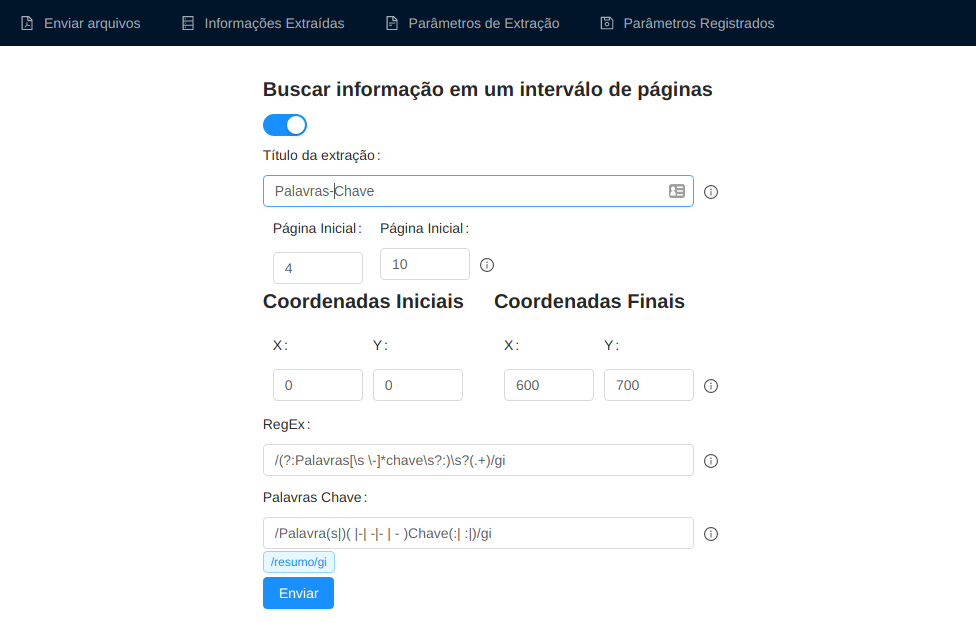
\includegraphics[width=1\textwidth]{figs/tccExtract/params2.png}
% \footnotesize Fonte: Autoria Própria
% \end{figure}

Os parâmetros registrados podem ser consultados na próxima aba, como apresentado na \textbf{Figura \ref{paramsR}}, lá a informação é recuperada do banco de dados e é possível remover um registro, caso desejado.

\begin{figure}[H]
\centering
\captionsetup{justification   = raggedright,
              singlelinecheck = false}
\caption{Parâmetros Registrados - Sistema de Extração de dados de TCC}\label{paramsR}
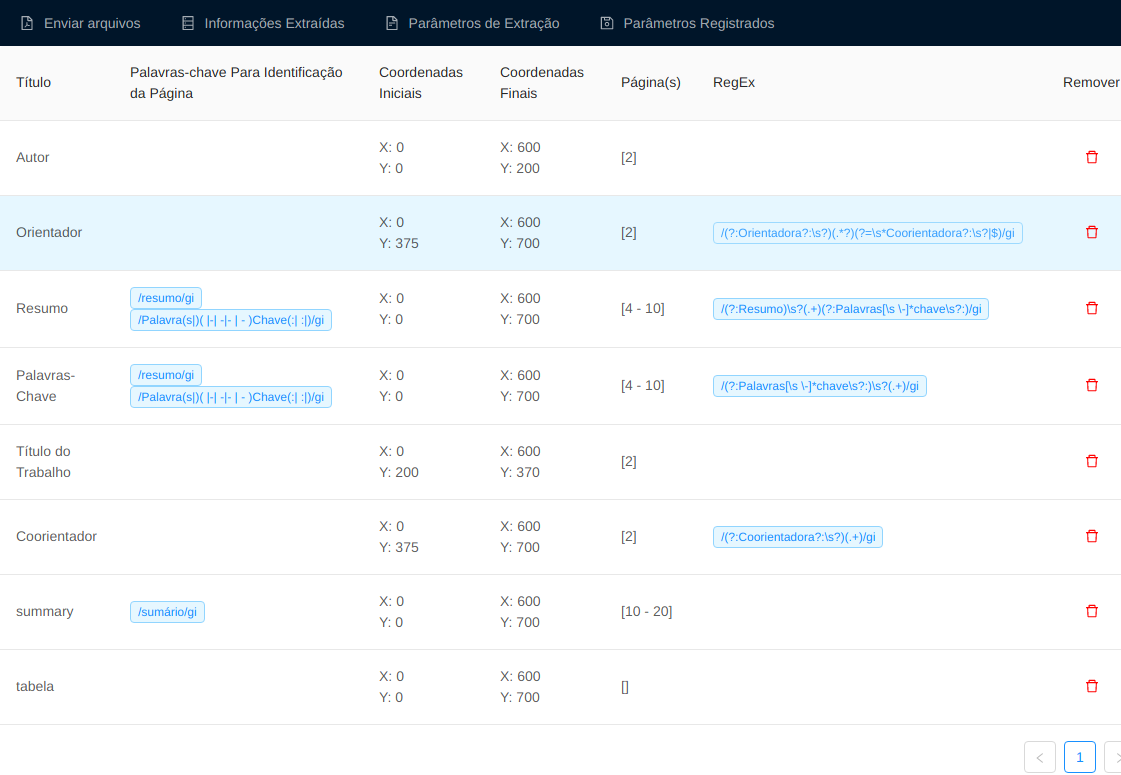
\includegraphics[width=1\textwidth]{figs/tccExtract/paramsR2.png}
\footnotesize Fonte: Autoria Própria
\end{figure}

Com os parâmetros devidamente registrados, é possível submeter novos arquivos, na \textbf{Figura \ref{upload}} o botão de upload apresentado aceita um ou mais arquivos PDF, mas respeitando uma das constrições de API RESTful, é feita apenas uma requisição para cada arquivo.

\begin{figure}[H]
\centering
\captionsetup{justification   = raggedright,
              singlelinecheck = false}
\caption{Envio de Arquivos - Sistema de Extração de dados de TCC}\label{upload}
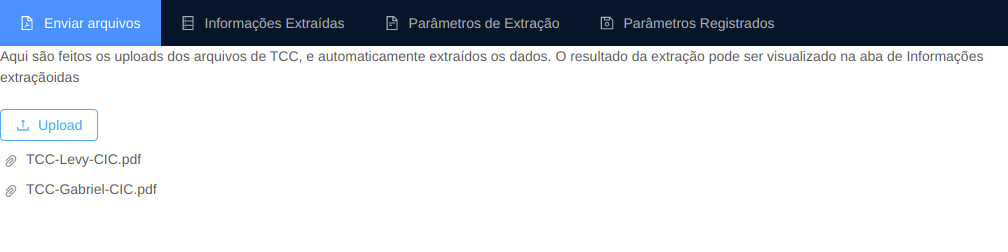
\includegraphics[width=1\textwidth]{figs/tccExtract/upload.png}
\footnotesize Fonte: Autoria Própria
\end{figure}

Após enviado, o resultado da extração pode ser consultado na aba seguinte. A tabela apresentada na \textbf{Figura \ref{extr}} é montada de acordo com os parâmetros que foram definidos como primordiais para o projeto de egressos.

Havendo mais informações extraídas, estas podem ser acessadas no formato de objeto JSON através do botão \textit{Mais} a direita. E o resumo no botão presente à esquerda.

\begin{figure}[H]
\centering
\captionsetup{justification   = raggedright,
              singlelinecheck = false}
\caption{Informações Extraídas - Sistema de Extração de dados de TCC}\label{extr}
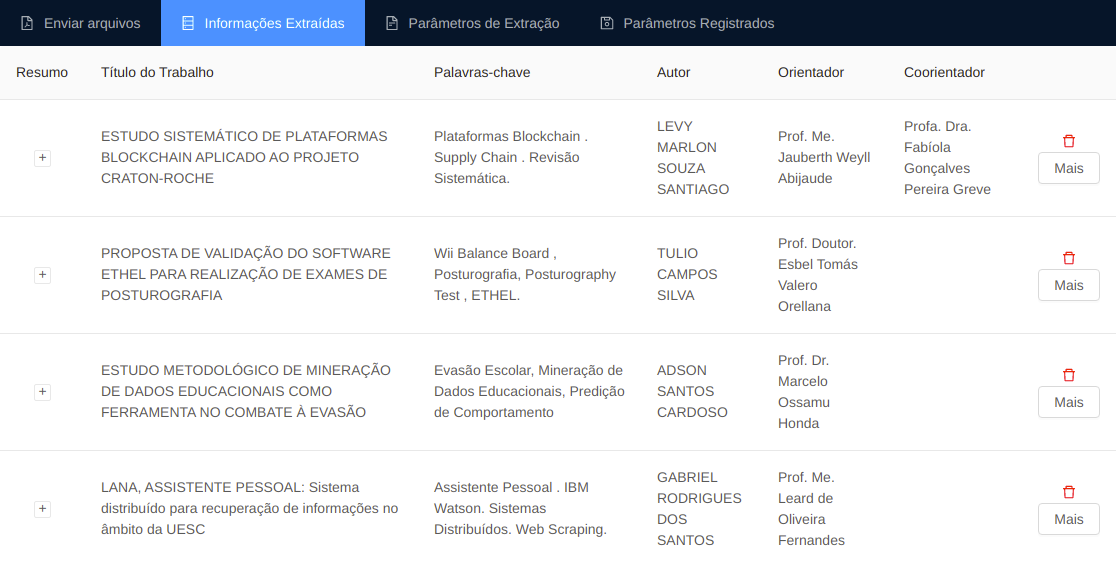
\includegraphics[width=1\textwidth]{figs/tccExtract/extr.png}
\footnotesize Fonte: Autoria Própria
\end{figure}
\chapter{Conclusões e Trabalhos Futuros}

Com o objetivo de realizar um estudo de validação do ETHEL, \textit{software} desenvolvido por uma equipe de pesquisadores e programadores da UESC. É apresentada neste trabalho uma metodologia de validação baseada em um estudo comparativo. Com esta finalidade se analisou a utilização do \textit{software} \textit{Posturography Test}, por ser uma solução que também utiliza a WBB na implementação de de exames posturográficos, e por já ter sido validado (\citeauthor{llorens2016posturography}, \citeyear{llorens2016posturography}). Além disso, está disponível de forma gratuita para uso. A metodologia  de validação, consiste na realização de testes com um mesmo grupo de pessoas. Na efetivação dos testes, deve ser utilizada a mesma WBB como plataforma de força e os pacientes devem executar a mesma sequência de testes em ambos os \textit{softwares} e, em condições semelhantes. Com isso, se ao fim dos testes, os dados coletados com os \textit{softwares} apresentarem uma correlação aceitável, pode-se inferir que o ETHEL apresenta dados válidos. 

Para viabilizar o estudo comparativo, o presente estudo  analisou as métricas estimadas no \textit{Posturography Test}. Após análise, foi constado que a Excursão Máxima AP e a Excursão máxima ML, que são utilizadas no \textit{Posturography Test}, não estavam implementadas no ETHEL. Sendo assim passaram ser calculadas e foram incluídas no conjunto de métricas do mesmo. 

A interface gráfica do modulo LOS foi desenvolvida e está funcional. Além disso, já é possível realizar a captura do deslocamento do COP do participante, que desloca o seu centro de massa sobre a WBB na direção do alvo indicado. Entretanto, as métricas calculadas a partir do LOS. (tempo de reação, excursão máxima e controle direcional) ainda não são estimadas pelo ETHEL. Esta limitação se deve à falta de descrição clara para realização do cálculo das mesmas, principalmente no \textit{Posturography Test}, ferramenta utilizada na proposta de validação do ETHEL.

Na realização dos testes com humanos, apresentados neste trabalho, O ETHEL apresentou excelente funcionamento. O que sugere que após o termino da implementação do módulo LOS, ele já estará pronto para execução da proposta de validação descrita. Ademais, o grupo de pesquisadores que cederam os dados dos testes apresentados, relataram que o ETHEL mostrou uma redução significativa no tempo de execução do exames, quando comparado com os testes preliminares feitos com o \textit{Posturography Test}. O que pode se tornar um fator decisivo na escolha de utilização entre os dois \textit{softwares}. Além disso, o mesmo grupo de voluntários deveria ser submetido a avaliação semelhante utilizando o \textit{Posturography Test}, possibilitando assim, ter uma prévia da eficácia da metodologia de de validação proposta. Entretanto, por indisponibilidade no sistema WEB esta etapa da avaliação não foi possível realizar o estudo comparando as duas aplicações. 

Visando aprimorar o protocolo de execução de aquisição dos dados e a redução do tempo na realização dos exames, ao fim dos testes, foi calculado o desvio da primeira repetição de cada condição em relação a média das repetições da condição em questão, na forma de erro relativo. Conforme os resultados apresentados no \textbf{\textbf{Capitulo} \ref{resultados}}, a métrica velocidade média apresentou um desvio da primeira repetição em relação a média das repetições, menor que 10\%. Além do mais, apresentou um desvio padrão médio próximo a zero. Isso pode indicar a não necessidade de realização de três repetições, quando se desejar estimar a velocidade média do COP. Principalmente na condição sensorial olhos fechados sem espuma, que foi a condição sensorial em que se apresentou melhores resultados. Entretanto, não é possível inferir que não se faz necessária a realização de três repetições para cada condição na realização dos testes. Pois, o estudo em questão realizou os testes com uma amostra pequena de pacientes. 


Como possíveis trabalhos futuros pode-se destacar o desenvolvimento e a integração ao ETHEL dos cálculos das métricas no módulo LOS. Deve-se realizar, também, testes com uma amostra maior de pacientes, visando aprimorar o protocolo de execução de aquisição dos dados e verificar a necessidade de realização de repetições para cada condição no cumprimento dos testes. Finalmente deve ser  realizado o estudo comparativo aqui proposto, como o objetivo de validar os resultados obtidos com o ETHEL. 
  
%O presente estudo analisou as métricas estimadas no Posturography Test. Após análise, foi constado que a Excursão Máxima AP e a Excursão máxima ML eram métricas que estavam presentes no Posturography Test, mas não pertenciam ao ETHEL. Sendo assim passaram ser calculadas e foram incluídas no mesmo. 

%A interface gráfica do modulo LOS foi desenvolvida e está funcional. Além disso, já é possível realizar a captura do deslocamento do COP do participante, que desloca o seu centro de massa sobre a WBB na direção do alvo indicado. Entretanto, as medidas apresentadas como resultado (tempo de reação, excursão máxima e controle direcional) ainda não são estimadas pelo ETHEL, devido a falta de descrição clara para realização do cálculo das mesmas, principalmente no Posturography Test ferramenta utilizada na proposta de validação do ETHEL.

%Visando aprimorar o protocolo de execução de aquisição dos dados e a redução do tempo na realização dos exames. Ao fim dos testes, foi calculado o desvio da primeira repetição de cada condição em relação a média das repetições da condição em questão, na forma de erro relativo. Conforme os resultados apresentados na Tabela \ref{tabelaResultados}, 51,85\% dos exames apresentaram um desvio da primeira repetição com a média das repetições, menor que 10\%. No entando, não é possível inferir que não se faz necessária a realização de três repetição para cada condição na realização dos testes. Pois, o estudo em questão realizou os testes com uma amostra pequena de pacientes. E uma análise de distribuição de Frequência em Intervalo de Classe deve ser feita para cada uma das quatro condições, afim de detalhar a distribuição dos erros de acordo com as condições sensoriais. 

%A proposta de validação para o software ETHEL é a realização do estudo comparativo com o software Posturography Test. Ele foi escolhido por ser uma solução que também utiliza a WBB na realização de exames posturográficos e por já ter sido validado (\cite{llorens2016posturography}, \citeyear{llorens2016posturography}). Além disso, está disponível de forma gratuita. A metodologia  de validação, consiste na realização de testes com um mesmo grupo de pessoas. Na realização dos testes, as pessoas utilizaram a mesma WBB como plataforma de força e executaram a mesma sequência de testes em ambos os softwares e, em condições semelhantes. Com isso, se ao fim dos teste, os dados coletados com os softwares apresentarem uma correlação aceitável, podemos inferir que o ETHEL apresenta dados válidos.           

%Na realização dos testes com humanos, apresentados neste trabalho. O ETHEL apresentou excelente funcionamento. O que sugere que após o termino da implementação do módulo LOS, ele já estará pronto para execução da proposta de validação descrita. Ademais, o grupo de pesquisadores que cederam os dados dos testes apresentados, relataram que o ETHEL mostrou uma redução significativa no tempo de execução do exames, quando comparado com o Posturography Test. O que pode se tornar um fator decisivo na escolha de utilização entre os dois softwares.

%Possíveis trabalhos futuros são:
%\begin{enumerate}
%    \item Desenvolver e integrar os cálculos das métricas no módulo LOS;
%    \item Realizar testes com uma amostra maior de pacientes, visando aprimorar o protocolo de execução de aquisição dos dados e verificar a necessidade de realização de repetições para cada condição no cumprimento dos testes.
%    \item Efetuação da proposta de validação descrita neste trabalho.
%\end{enumerate}
  

%\chapter{Conclusão}




% ----------------------------------------------------------
% Finaliza a parte no bookmark do PDF
% para que se inicie o bookmark na raiz
% e adiciona espaço de parte no Sumário
% ----------------------------------------------------------
\phantompart

% ---
% Conclusão
% ---
%\chapter{Conclusão}
% ---

% ----------------------------------------------------------
% ELEMENTOS PÓS-TEXTUAIS
% ----------------------------------------------------------
\postextual
% ----------------------------------------------------------

% ----------------------------------------------------------
% Referências bibliográficas
% ----------------------------------------------------------
\bibliography{TCC.bib}

% ----------------------------------------------------------
% Glossário
% ----------------------------------------------------------
%
% Consulte o manual da classe abntex2 para orientações sobre o glossário.
%
%\glossary

% ----------------------------------------------------------
% Apêndices
% ----------------------------------------------------------

% ---
% Inicia os apêndices
% ---
\begin{apendicesenv}

% Imprime uma página indicando o início dos apêndices
\partapendices

% ----------------------------------------------------------
\chapter{Resultados dos Testes}\label{resultadostestes}

Na tabela a seguir, são apresentados os resultados das métricas estimadas, velocidade média, excursão máxima AP e  excursão máxima ML, de cada participante. Nos testes foram realizadas três repetições para cada condição sensorial (olhos abertos em uma superfície plana (OASP), olhos fechados em uma superfície plana (OFSP), olhos abertos sobre a espuma (OASE) e olhos fechados sobre a espuma (OFSE)). A média das repetições de cada condição sensorial pode ser vista na terceira coluna da tabela. Na quarta coluna é apresentado o desvio padrão das três repetições. Na quinta coluna é apresentado o erro relativo entre a primeira repetição e a média das três repetições.   
% ----------------------------------------------------------
\begin{table}[ht]
\captionsetup{justification   = raggedright,
              singlelinecheck = false}
\caption{Resultados dos testes }
% {Resultados dos testes (OASP - Olhos abertos em uma superfície plana. OFSP - Olhos fechados em uma superfície plana. OASE - Olhos abertos sobre a espuma. OFSE - Olhos fechados sobre a espuma.)}

\begin{flushright}
(continua)
\end{flushright}
\begin{tabular}{|c|c|c|c|c|c|}
\hline
\textbf{Paciente}   & \textbf{Teste}                             & \textbf{Condição} & \textbf{Média} & \textbf{Desvio} & \textbf{Erro} \\
& & & & \textbf{Padrão} & \textbf{(\%)} \\ \hline
\multirow{12}{*}{1} & \multirow{4}{*}{Velocidade Média (cm/seg)} & OASP\footnotemark{} & 1,18 & 0,10 & 9,42 \\ \cline{3-6} 
 &  & OFSP\footnotemark{} & 1,30 & 0,03 & 0,97 \\ \cline{3-6} 
 &  & OASE\footnotemark{} & 1,76 & 0,09 & 5,20 \\ \cline{3-6} 
 &  & OFSE\footnotemark{} & 2,60 & 0,23 & 9,75 \\ \cline{2-6} 
 & \multirow{4}{*}{Excursão Máxima AP (cm)} & OASP & 0,69 & 0,28 & 42,28 \\ \cline{3-6} 
 &  & OFSP & 0,94 & 0,12 & 2,87 \\ \cline{3-6} 
 &  & OASE & 1,66 & 0,48 & 8,95 \\ \cline{3-6} 
 &  & OFSE & 2,66 & 0,44 & 10,89 \\ \cline{2-6} 
 & \multirow{4}{*}{Excursão Máxima ML (cm)} & OASP & 1,70 & 0,21 & 12,16 \\ \cline{3-6} 
 &  & OFSP & 1,57 & 0,71 & 49,68 \\ \cline{3-6} 
 &  & OASE & 3,31 & 0,40 & 13,05 \\ \cline{3-6} 
 &  & OFSE & 4,21 & 0,60 & 14,01 \\ \hline
\end{tabular}
\end{table}
\pagebreak

% PARTE 2

\begin{table}[ht]
\begin{flushleft}
Tabela \ref{resultadostestes} - Resultados dos testes
\begin{flushright}
(continua)
\end{flushright}
\end{flushleft}
%\caption{Resultados testes}
%\label{resultadostestes}
\begin{tabular}{|c|c|c|c|c|c|}
\hline
\textbf{Paciente}   & \textbf{Teste}                             & \textbf{Condição} & \textbf{Média} & \textbf{Desvio} & \textbf{Erro} \\
& & & & \textbf{Padrão} & \textbf{(\%)} \\ \hline
\multirow{12}{*}{2} & \multirow{4}{*}{Velocidade Média (cm/seg)} & OASP & 1,41 & 0,24 & 18,67 \\ \cline{3-6} 
 &  & OFSP & 1,59 & 0,15 & 7,29 \\ \cline{3-6} 
 &  & OASE & 1,97 & 0,23 & 11,66 \\ \cline{3-6} 
 &  & OFSE & 3,82 & 0,59 & 3,47 \\ \cline{2-6} 
 & \multirow{4}{*}{Excursão Máxima AP (cm)} & OASP & 1,22 & 0,32 & 20,58 \\ \cline{3-6} 
 &  & OFSP & 1,54 & 0,25 & 16,15 \\ \cline{3-6} 
 &  & OASE & 1,91 & 0,44 & 17,61 \\ \cline{3-6} 
 &  & OFSE & 2,99 & 0,40 & 14,64 \\ \cline{2-6} 
 & \multirow{4}{*}{Excursão Máxima ML (cm)} & OASP & 2,79 & 0,19 & 7,50 \\ \cline{3-6} 
 &  & OFSP & 2,82 & 0,78 & 30,53 \\ \cline{3-6} 
 &  & OASE & 2,77 & 0,43 & 1,77 \\ \cline{3-6} 
 &  & OFSE & 5,32 & 1,33 & 28,79 \\ \hline
\multirow{12}{*}{3} & \multirow{4}{*}{Velocidade Média (cm/seg)} & OASP & 1,28 & 0,05 & 3,27 \\ \cline{3-6} 
 &  & OFSP & 1,35 & 0,08 & 4,75 \\ \cline{3-6} 
 &  & OASE & 1,62 & 0,39 & 13,39 \\ \cline{3-6} 
 &  & OFSE & 1,87 & 0,13 & 7,61 \\ \cline{2-6} 
 & \multirow{4}{*}{Excursão Máxima AP (cm)} & OASP & 1,24 & 0,17 & 11,46 \\ \cline{3-6} 
 &  & OFSP & 1,18 & 0,16 & 2,07 \\ \cline{3-6} 
 &  & OASE & 1,66 & 0,25 & 13,13 \\ \cline{3-6} 
 &  & OFSE & 1,42 & 0,04 & 2,36 \\ \cline{2-6} 
 & \multirow{4}{*}{Excursão Máxima ML (cm)} & OASP & 2,19 & 0,26 & 12,96 \\ \cline{3-6} 
 &  & OFSP & 2,92 & 0,43 & 11,64 \\ \cline{3-6} 
 &  & OASE & 3,19 & 0,78 & 2,97 \\ \cline{3-6} 
 &  & OFSE & 4,26 & 0,89 & 21,45 \\ \hline
\multirow{12}{*}{4} & \multirow{4}{*}{Velocidade Média (cm/seg)} & OASP & 1,10 & 0,02 & 2,05 \\ \cline{3-6} 
 &  & OFSP & 1,20 & 0,03 & 1,67 \\ \cline{3-6} 
 &  & OASE & 1,42 & 0,16 & 12,53 \\ \cline{3-6} 
 &  & OFSE & 2,18 & 0,37 & 18,18 \\ \cline{2-6} 
 & \multirow{4}{*}{Excursão Máxima AP (cm)} & OASP & 0,79 & 0,12 & 9,99 \\ \cline{3-6} 
 &  & OFSP & 0,74 & 0,09 & 13,59 \\ \cline{3-6} 
 &  & OASE & 1,63 & 0,40 & 22,72 \\ \cline{3-6} 
 &  & OFSE & 2,10 & 0,93 & 3,47 \\ \cline{2-6} 
 & \multirow{4}{*}{Excursão Máxima ML (cm)} & OASP & 2,20 & 0,35 & 12,48 \\ \cline{3-6} 
 &  & OFSP & 2,27 & 0,43 & 10,81 \\ \cline{3-6} 
 &  & OASE & 3,14 & 0,24 & 3,37 \\ \cline{3-6} 
 &  & OFSE & 4,82 & 1,80 & 28,24 \\ \hline

\end{tabular}
\end{table}
\pagebreak

% PARTE 3

\begin{table}[ht]
\begin{flushleft}
Tabela \ref{resultadostestes} - Resultados dos testes
\begin{flushright}
(continua)
\end{flushright}
\end{flushleft}
%\caption{Resultados testes}
%\label{resultadostestes}
\begin{tabular}{|c|c|c|c|c|c|}
\hline
\textbf{Paciente}   & \textbf{Teste}                             & \textbf{Condição} & \textbf{Média} & \textbf{Desvio} & \textbf{Erro} \\
& & & & \textbf{Padrão} & \textbf{(\%)} \\ \hline

\multirow{12}{*}{5} & \multirow{4}{*}{Velocidade Média (cm/seg)} & OASP & 1,07 & 0,09 & 6,53 \\ \cline{3-6} 
 &  & OFSP & 1,33 & 0,23 & 15,26 \\ \cline{3-6} 
 &  & OASE & 1,63 & 0,10 & 4,62 \\ \cline{3-6} 
 &  & OFSE & 2,48 & 0,25 & 10,86 \\ \cline{2-6} 
 & \multirow{4}{*}{Excursão Máxima AP (cm)} & OASP & 1,55 & 0,27 & 0,83 \\ \cline{3-6} 
 &  & OFSP & 1,58 & 0,33 & 15,93 \\ \cline{3-6} 
 &  & OASE & 2,21 & 0,40 & 3,54 \\ \cline{3-6} 
 &  & OFSE & 2,15 & 0,61 & 2,65 \\ \cline{2-6} 
 & \multirow{4}{*}{Excursão Máxima ML (cm)} & OASP & 2,41 & 0,19 & 6,84 \\ \cline{3-6} 
 &  & OFSP & 3,11 & 0,30 & 9,67 \\ \cline{3-6} 
 &  & OASE & 3,04 & 0,62 & 14,67 \\ \cline{3-6} 
 &  & OFSE & 3,85 & 0,66 & 13,70 \\ \hline
\multirow{12}{*}{6} & \multirow{4}{*}{Velocidade Média (cm/seg)} & OASP & 1,66 & 0,08 & 5,61 \\ \cline{3-6} 
 &  & OFSP & 1,88 & 0,11 & 6,41 \\ \cline{3-6} 
 &  & OASE & 1,81 & 0,13 & 0,95 \\ \cline{3-6} 
 &  & OFSE & 2,68 & 0,33 & 0,64 \\ \cline{2-6} 
 & \multirow{4}{*}{Excursão Máxima AP (cm)} & OASP & 1,38 & 0,11 & 8,85 \\ \cline{3-6} 
 &  & OFSP & 1,57 & 0,18 & 12,92 \\ \cline{3-6} 
 &  & OASE & 1,62 & 0,27 & 7,59 \\ \cline{3-6} 
 &  & OFSE & 1,70 & 0,27 & 14,75 \\ \cline{2-6} 
 & \multirow{4}{*}{Excursão Máxima ML (cm)} & OASP & 3,25 & 0,60 & 14,01 \\ \cline{3-6} 
 &  & OFSP & 3,14 & 0,66 & 13,07 \\ \cline{3-6} 
 &  & OASE & 2,42 & 0,25 & 11,13 \\ \cline{3-6} 
 &  & OFSE & 4,63 & 0,54 & 6,14 \\ \hline
\multirow{12}{*}{7} & \multirow{4}{*}{Velocidade Média (cm/seg)} & OASP & 0,87 & 0,09 & 7,97 \\ \cline{3-6} 
 &  & OFSP & 1,04 & 0,06 & 6,33 \\ \cline{3-6} 
 &  & OASE & 1,09 & 0,10 & 4,24 \\ \cline{3-6} 
 &  & OFSE & 1,82 & 0,14 & 5,31 \\ \cline{2-6} 
 & \multirow{4}{*}{Excursão Máxima AP (cm)} & OASP & 0,84 & 0,33 & 17,40 \\ \cline{3-6} 
 &  & OFSP & 0,52 & 0,13 & 16,36 \\ \cline{3-6} 
 &  & OASE & 1,00 & 0,25 & 14,55 \\ \cline{3-6} 
 &  & OFSE & 1,48 & 0,13 & 4,64 \\ \cline{2-6} 
 & \multirow{4}{*}{Excursão Máxima ML (cm)} & OASP & 1,85 & 0,19 & 8,18 \\ \cline{3-6} 
 &  & OFSP & 2,07 & 0,23 & 12,82 \\ \cline{3-6} 
 &  & OASE & 1,90 & 0,30 & 0,95 \\ \cline{3-6} 
 &  & OFSE & 3,26 & 0,29 & 6,82 \\ \hline


\end{tabular}
\end{table}
\pagebreak

% PARTE 4

\begin{flushleft}
Tabela \ref{resultadostestes} - Resultados dos testes
\end{flushleft}

\begin{flushright}
(conclusão)
\end{flushright}

\begin{table}[ht]
%\caption{Resultados testes}
%\label{resultadostestes}
\begin{tabular}{|c|c|c|c|c|c|}
\hline
 \textbf{Paciente}   & \textbf{Teste}                             & \textbf{Condição} & \textbf{Média} & \textbf{Desvio} & \textbf{Erro} \\
& & & & \textbf{Padrão} & \textbf{(\%)} \\ \hline

\multirow{12}{*}{8} & \multirow{4}{*}{Velocidade Média (cm/seg)} & OASP & 1,21 & 0,12 & 6,42 \\ \cline{3-6} 
 &  & OFSP & 1,35 & 0,09 & 2,63 \\ \cline{3-6} 
 &  & OASE & 1,56 & 0,07 & 4,86 \\ \cline{3-6} 
 &  & OFSE & 2,53 & 0,34 & 15,60 \\ \cline{2-6} 
 & \multirow{4}{*}{Excursão Máxima AP (cm)} & OASP & 1,60 & 0,45 & 1,27 \\ \cline{3-6} 
 &  & OFSP & 1,38 & 0,43 & 19,27 \\ \cline{3-6} 
 &  & OASE & 2,24 & 0,75 & 8,39 \\ \cline{3-6} 
 &  & OFSE & 3,08 & 1,41 & 47,21 \\ \cline{2-6} 
 & \multirow{4}{*}{Excursão Máxima ML (cm)} & OASP & 2,28 & 0,64 & 31,49 \\ \cline{3-6} 
 &  & OFSP & 2,64 & 0,73 & 20,94 \\ \cline{3-6} 
 &  & OASE & 2,43 & 0,47 & 7,39 \\ \cline{3-6} 
 &  & OFSE & 3,96 & 0,86 & 24,55 \\ \hline
\multirow{12}{*}{9} & \multirow{4}{*}{Velocidade Média (cm/seg)} & OASP & 0,96 & 0,08 & 7,51 \\ \cline{3-6} 
 &  & OFSP & 1,19 & 0,05 & 4,58 \\ \cline{3-6} 
 &  & OASE & 1,36 & 0,26 & 21,15 \\ \cline{3-6} 
 &  & OFSE & 1,97 & 0,24 & 14,08 \\ \cline{2-6} 
 & \multirow{4}{*}{Excursão Máxima AP (cm)} & OASP & 0,87 & 0,23 & 30,47 \\ \cline{3-6} 
 &  & OFSP & 1,00 & 0,40 & 30,35 \\ \cline{3-6} 
 &  & OASE & 1,23 & 0,24 & 22,67 \\ \cline{3-6} 
 &  & OFSE & 1,88 & 0,36 & 21,70 \\ \cline{2-6} 
 & \multirow{4}{*}{Excursão Máxima ML (cm)} & OASP & 1,46 & 0,37 & 21,54 \\ \cline{3-6} 
 &  & OFSP & 2,12 & 0,77 & 6,66 \\ \cline{3-6} 
 &  & OASE & 2,07 & 0,76 & 41,99 \\ \cline{3-6} 
 &  & OFSE & 4,56 & 0,80 & 13,96 \\ \hline
\end{tabular}
\end{table}
\addtocounter{footnote}{-4} %4=n
\stepcounter{footnote}\footnotetext{Olhos abertos em uma superfície plana (OASP)}
\stepcounter{footnote}\footnotetext{Olhos fechados em uma superfície plana (OFSP)}
\stepcounter{footnote}\footnotetext{Olhos abertos sobre a espuma (OASE)}
\stepcounter{footnote}\footnotetext{Olhos fechados sobre a espuma (OFSE)}


% ----------------------------------------------------------

% ----------------------------------------------------------


\end{apendicesenv}
% ---

% % ----------------------------------------------------------
% % Anexos
% % ----------------------------------------------------------

% % ---
% % Inicia os anexos
% % ---
% \begin{anexosenv}

% % Imprime uma página indicando o início dos anexos
% \partanexos
% \chapter{Parecer do CEP } \label{anexoCEP} \title{Parece CEP UESC}
% '\includepdf[pages=-]{CEP.pdf}
% % ---
% \end{anexosenv}

%---------------------------------------------------------------------
% INDICE REMISSIVO
%---------------------------------------------------------------------
\phantompart
\printindex
%---------------------------------------------------------------------

\end{document}
